%\documentclass{article}
\documentclass[12pt]{report}
\linespread{1.5}

%% Useful packages
\usepackage[a4paper,top=3cm,bottom=3cm,left=3.5cm,right=3cm,marginparwidth=1.75cm]{geometry}
\usepackage{amsmath}
\usepackage{cite}
\usepackage{courier}
\usepackage{caption}
\usepackage{graphicx}
\usepackage[colorinlistoftodos]{todonotes}
\usepackage[colorlinks=true, allcolors=blue]{hyperref}
\usepackage{float}
\usepackage{setspace}
\usepackage{subfigure}
\usepackage{url}
\usepackage{tabularx}
\usepackage[utf8]{inputenc}
\usepackage{mathptmx} %Times Font
\usepackage{mathrsfs}
\usepackage{enumerate}
\usepackage{paralist}
\usepackage{mdwlist}
\usepackage{ulem}
\usepackage{threeparttable}
\usepackage{bm}
\usepackage{listings}
%\usepackage[framed,numbered,autolinebreaks,useliterate]{mcode}
\usepackage{xcolor}

\usepackage{amsmath}
\DeclareMathOperator*{\argmax}{arg\,max}
\DeclareMathOperator*{\argmin}{arg\,min}

%tikz settings
\usepackage{tikz}
\usetikzlibrary{shapes.geometric}
\usetikzlibrary{arrows.meta,arrows}
\tikzstyle{decision} = [diamond, draw, fill=blue!20, 
text width=6em, text badly centered, node distance=3cm, inner sep=0pt]
\tikzstyle{block} = [rectangle, draw, fill=white, 
text width=9em, text centered, rounded corners, minimum height=4em]
\tikzstyle{block2} = [rectangle, draw, fill=yellow!20, 
text width=9em, text centered, rounded corners, minimum height=4em]
\tikzstyle{line} = [draw, -latex']
\tikzstyle{cloud} = [draw, ellipse,fill=red!20, node distance=3cm,
minimum height=4em]

\newcommand{\tabincell}[2]{\begin{tabular}{@{}#1@{}}#2\end{tabular}}
\newif\ifoutputscaleerror\outputscaleerrorfalse


\begin{document}

%==== FRONT PART====
\begin{titlepage}

\begin{figure}[H]
\centering

\includegraphics[scale=0.8]{Title/logo.eps}
\caption*{}
\label{fig:entropy} 
\end{figure}

\centering
\LARGE{\textbf{Place Recognition and Localization for Multi-Robot SLAM}}\\[2in]



\large{\textbf{Liu Xiangyu}}\\[1in]

\textbf{SCHOOL OF ELECTRICAL AND ELECTRONIC ENGINEERING}

\textbf{MASTER OF SCIENCE IN COMPUTER CONTROL AND AUTOMATION}\\[0.25in]

\textbf{2019}
\newpage
\end{titlepage}

%\begingroup
%\let\cleardoublepage\clearpage
\pagenumbering{roman}
\tableofcontents
%\endgroup

%=== FRONT PART ===
%=== ABSTRCT ===

%\begin{center}
\chapter*{Abstract}
%\end{center}
\addcontentsline{toc}{chapter}{Abstract}

SLAM (Simultaneous Localization and Mapping) is an important component of robot systems, enabling robot systems to exploit and map an unknown environment, while estimating its own position. Single robot SLAM techniques based on monocular or stereo cameras, color or depth images and segmentation- or feature-based algorithms, have been considerable developed with many successful solutions proposed, during years of research. Compared to single robot SLAM, multi robot SLAM have several advantage e.g. robustness and quicker exploration. However, the development of multi robot SLAM is much slower, because of the difficulties such as determination of relative poses of robots and communication, etc. CORB-SLAM as a multi robot SLAM system, of which the clients are based on ORB-SLAM2, inheriting its advantages like low-cost sensors and low computation cost, has not been evaluated in a quantitative method to assess its performance. For multi robot SLAM, the adaptability in life-long scenarios is another important research topic, since multi robots may run in different dates and seasons.
This work quantitatively evaluates CORB-SLAM, and experiments to combine it with illumination variance algorithm to improve its performance under different illumination and season.


\par
\textbf{Keywords:} Multi-robot SLAM, CORB-SLAM, Quantitative Trajectory Evaluation, Life-long SLAM.

%=== END OF CHAPTER ONE ===

%=== FRONT PART ===
%=== ACKNOWLEDGEMENT ===

%\begin{center}
\chapter*{Acknowledgement}
%\end{center}
\addcontentsline{toc}{chapter}{Acknowledgement}

This dissertation is finished under the guidance of PhD students e.g. Zhang Jun, Peng Guohao, Yue Yufeng and Professor Wang Danwei, in ST Engineering-NTU ROBOTICS ADVANCe LABORATORY in NTU. I sincerely thank them and all other members in the lab for their patient and careful help during the implementation, experiment and compilation of the dissertation. Without their help on providing technical suggestions and possible solutions to the research objectives, and help during the collection of the related datasets, this dissertation project would not go so smoothly within two short semesters.


%=== END OF ACKNOWLEDGEMENT  ===

%%=== FRONT PART ===
%=== ACRONYMS ===

%\begin{center}
\chapter*{Acronyms}
%\end{center}
\addcontentsline{toc}{chapter}{Acronyms}

Acronyms goes here.

%=== END OF ACRONYMS ===

%%=== FRONT PART ===
%=== SYMBOLS ===

%\begin{center}
\chapter*{Symbols}
%\end{center}
\addcontentsline{toc}{chapter}{Symbols}

Symbols goes here.

%=== END OF ACKNOWLEDGEMENT  ===


\listoffigures 
\addcontentsline{toc}{chapter}{Lists of Figures}
\newpage

\listoftables 
\addcontentsline{toc}{chapter}{Lists of Tables}
\newpage


%==== MAIN PART ====
\pagenumbering{arabic}
%=== CHAPTER ONE (1) ===
%=== INTRODUCTION ===

\chapter{Introduction}

\section{Background}

SLAM(Simultaneous localization and mapping) is an important component in developing mobile autonomous systems. It enable a vehicle the ability to explore and map an unknown environment, while at the same time estimating its own position in the environment, using only its sensors equipped onboard.

SLAM systems can be accomplished by both single or multiple robots. Multiple-robot SLAM or MRSLAM, offer several advantages compared to single robot SLAM, for example:
\begin{itemize}
	\item Robustness to failure of single robots,
	\item Faster environment exploration in time critical Search and Rescue(SaR) mission.
\end{itemize} 


However, Adapting SLAM technology to multiple-robot scenario brings some new changes as identified by Saeedi et al \cite{saeedi2016multiple}:
\begin{itemize}
	\item Relative Poses of Robots. The map created by each robot in MR-SLAM systems in its own reference is called the local map. It is a difficult task to merge all the local client maps created by each robot to create a globally consistent map of the environment, as the required transformation or alignment matrices that relate these maps to each other are generally unknown. 
	\item Closing Loops. Loop closure is defined as identifying a previously observed but not very recent place. Solving this problem for a multiple robot cluster requires taking advantage of all information resources from each client. In multi-robot SLAM, different events can trigger loop closure, such as direct or indirect robots encounter, when robots see the same area of features worldwide. 
	\item Communications. Multi-robot SLAM requires a medium to be highly available for data sharing between robots. It is possible to exchange information between robots via communication channels. The quality of the channels of communication depends on the environment. Communication, for example, is a challenging issue for a robots team in underwater environments, where the environment imposes limitations on data rate and bandwidth. 
\end{itemize}

Because of the limitation of the difficulties mentioned above, the development of multiple-robot SLAM is much slower than single-robot SLAM. Finding a solution to these problem will push the adaption of SLAM technology to a new level.

\begin{figure}
	\centering
	\subfigure[Input image and extracted keypoints.]{
		\begin{minipage}[t]{0.4\linewidth}
			\centering
			\includegraphics[width=2in]{Chapter1/introimg.eps}
			%\caption{fig1}
		\end{minipage}
	}
	\subfigure[Mapping result.]{
		\begin{minipage}[t]{0.4\linewidth}
			\centering
			\includegraphics[width=2in]{Chapter1/intromap.eps}
			%\caption{fig2}
		\end{minipage}
	}
	\caption{A demonstration of input and mapping results of SLAM systems}
	\label{fig:backgroundslam}
\end{figure}

\section{Motivation and Objectives}

Recently, some solutions for multi-robot SLAM systems have been proposed. One of them is CORB-SLAM proposed in \cite{li2017corb}. As its clients based on ORB-SLAM, it inherits major advantages of ORB-SLAM e.g. relatively low computational cost and low cost of sensors. But in its initial work, the accuracy of its map fusion results are not evaluated in a quantitative evaluation method, while only a rough demonstration of its mapping results is given. Therefore, quantitative evaluation of CORB-SLAM with mapping results of single-robot ORB-SLAM system and CORB-SLAM clients given for comparison can help understand the performance of this multi-robot slam algorithm and assess the feasibility of its potential applications.

Another critical requirement of applications of multi-robot slam algorithms is its ability to fuse sub maps under different illumination conditions and season, which is named as life-long application circumstances. Illumination variance method proposed in \cite{maddern2014illumination}  with advantages of easy implement and low computational cost, may be able to help CORB-SLAM to deal with illumination and season changes. Therefore related experiments are undertaken in this work in order to find a effective way to combine CORB-SLAM with illumination variance.

\section{Major contribution of the Dissertation}
\begin{enumerate}[1.]
	\item Evaluation of CORB-SLAM on several datasets with quantitative trajectory evaluation results provided.
	\item Experiment of combination of CORB-SLAM with illumination variance algorithm to test whether illumination variance method is suitable to enhance ability of CORB-SLAM to deal with illumination changes.
\end{enumerate}

\section{Organisation of the Dissertation}
This dissertation is organised into several chapters:
\begin{enumerate}[1.]
	\item Chapter 2 briefly outlines the development of visual SLAM technique. Firstly, the classic structure of visual SLAM system is introduced, and the critical algorithms involved are elaborated, so as the classifications of visual SLAM systems. Then two main algorithms involved in this work, ORB-SLAM and CORB-SLAM, are demonstrated. This chapter also explores prior work in shade dealing algorithms required to implement life-long SLAM.
	
	\item Chapter 3 explains the methodology used in this dissertation to evaluate map fusion performance of CORB-SLAM, and how to combine illumination variance method with CORB-SLAM system to test if illumination variance can be utilized to enhance the ability of CORB-SLAM to deal with illumination changes.
	
	\item Chapter 4 shows the results of 
	
	\begin{inparaenum}[(a)]
		\item the evaluation of CORB-SLAM on selected 2 datasets including 
		\begin{inparaenum}[(i)]
			\item KITTI Visual Odometry Dataset \cite{Geiger2012CVPR},
			\item NTU Dataset \cite{zhang2018two},
		\end{inparaenum}
	
		\item the evaluation of CORB-SLAM combined with illumination variance on Oxford RobotCar Dataset \cite{maddern20171}.
		\end{inparaenum}
		
	\item Chapter 5 analysis the results demonstrated in chapter 4 in detail, discussing the improvement and the disadvantages.
	
	\item Chapter 6 concludes the work done in this dissertation, and comments on some limitation and drawbacks of algorithms used in this work, which future work need focus on.  

\end{enumerate}


%=== END OF CHAPTER ONE ===
\newpage



%=== CHAPTER TWO (2) ===
%=== Literature Review ===

\chapter{Literature Review}

\section{Visual SLAM}

\subsection{Introduction}
Simultaneous Localizaiton and Mapping (SLAM) is a technique for obtaining an unknown environment's 3D structure and sensor movement in the environment. Following years of development, SLAM-based application has become widespread, such as 3D modeling based on computer vision, self-driving cars and augmented reality(AR) visualization. 

In early SLAM algorithms, there exit many different modalities of sensors integrated in SLAM systems, such as rotary encoders, light detection and ranging radar (LiDAR), inertial sensors, GPS and cameras. In recent years, SLAM using cameras only,  specifically named as visual SLAM (vSLAM), has been actively discussed because of the simple, low-cost the sensor configuration, and  abundant information. But meanwhile this technique also brings more difficulties than others using integrated sensors\cite{taketomi2017visual}. 

vSLAM algorithms have proposed widely in the field of computer vision, robotics and AR. The low requirement on the modalities of sensors, requiring cameras only, is the major advantage of vSLAM technique, so that it is very suitable for low-cost unmanned vehicles, robots with limited load capacity and power supply like drones, or mobile devices such as camera-mounted tablets or smart phones.

However, the difficulties brought by vSLAM can not be ignored. Instead of obtaining depth and location information directly from LiDAR, GPS or depth camera in integrated SLAM systems, vSLAM technique needs to compute all these information from color or gray images, which reduces stability and accuracy for several estimation steps involved in this process. Also obviously the computational cost are significantly higher. Therefore, the problem of how to improve the performance and reduce computational cost of vSLAM has always been widely concerned.

%\subsection{Feature-based Algorithm}

%\subsection{Segmentation-based Algorithm}

\subsection{ORB-SLAM}
\label{chp:orbslam}
One of the state-of-the-art vSLAM solutions for single-robot systems is ORB-SLAM, initially proposed in \cite{mur2015orb}, and upgraded to a second version in \cite{mur2017orb}.

Initially proposed as a monocular SLAM system based on features, ORB-SLAM enables robots to map in real time small or large, indoor or outdoor environments with input of single camera images. The new vision has been upgraded to ORB-SLAM2 in \cite{mur2017orb} and can process monocular, stereo and RGB-D inputs. As stated in the proposed work \cite{mur2015orb}, ORB-SLAM is based on the main ideas of PTAM, the place recognition algorithm in \cite{galvez2012bags}, the use of covisibility information for large-scale operation \cite{strasdat2011double}, \cite{mei2010closing} and the scale-aware loop closure in \cite{strasdat2010scale}.  As a novel monocular SLAM system, the main contributions of ORB-SLAM are:
\begin{enumerate}[1.]
	\item In all tasks, the same features are used: tracking, mapping, closing of loops and relocation. Making the system more efficient, reliable and simple with the same features. And using ORB features enables GPU-free real-time performance, with signiticant invariance to changes in lighting and viewpoint. 
	\item In large environments, real-time performance. Due to the advantage of using a covisibility graph, the tracking and mapping modules are focused in a local visible area, independent of the global map. 
	\item Loop closing in real time. Optimizing a pose graph called the Essential Graph is adapted to perform the closing performance of the real-time loop. The Essential Graph is created from links to loop closures, strong edges in the covisibility graph, and a system maintained spanning tree. \item Real time camera relocation with exceptional viewpoint and illumination invariance. This improves the reuse of maps and also allows recovery from failure tracking. 
	\item A new robust and automatic initialization procedure 
	mode-selection-based that creates an initial map.
	\item A survival of the most appropriate approach to keyframe selection and map point, very restrictive in culling but generous in spawning. This policy enhances service life and improves the robustness of tracking because redundant key frames are discarded.
\end{enumerate}

ORB-SLAM system, see on Figure \ref{fig:orbslamoverview}, performs three threads that run in parallel: tracking, local mapping and loop closing. 

%The tracking thread is in charge of localizing the camera with every frame and deciding when to insert a new keyframe.	The module firstly match current frames with previous frames, and optimize the pose using motion-only bundle adjustment. If the 

\begin{figure}[H]
	\centering
	\includegraphics[width=5in]{Chapter2/ORBSLAMOverview.eps}
	\caption{ORB-SLAM system overview.}
	\label{fig:orbslamoverview} 
\end{figure}

\section{Multi-robot SLAM}

Multi-robot SLAM (MR-SLAM) uses several collaborative robots to map an unknown environment as an extended system of single-robot SLAM. However, the extension can not be easily implemented as each client maps their surroundings on their own local frame of reference. Therefore, in order to merge the sub map of several clients into a consistent global map, the map fusion server needs to be able to connect and find the transformation between different local client reference frames.The environment can be mapped significantly faster using MR-SLAM technique on a cluster of multi ground or hybrid robots and the uncertainty in the system can be reduced due to data redundancy.
Furthermore, if separate robots are equipped with heterogeneous sensors, the fused global map may contain much more feature information than a single robot map. Another obvious advantage is the robustness of one or more robots to fail, particularly when data is decentralized. 

As concluded in \cite{10.1007/978-3-319-78452-6_15}, besides the advantages above, MR-SLAM systems also face problems and choices in the following aspects:

\begin{inparaenum}[1.]
	\item Centralization or Decentralization. Determining where data processing takes place is one of the main questions building MR-SLAM systems. Data is processed in centralized approaches on a central server, performing the task to fuse  the information collected by all robots and distribut global map information to clients to improve their ability to self-locate\cite{forster2013collaborative, li2012laser,li2017corb}. By contrast, decentralized MR-SLAM systems usually have several clients, interconnected with each other and managed by a coordinating structure that allows systems to efficiently deal with large numbers of agents\cite{bresson2013consistent,fox2006distributed}. 
	
	\item Communication and information sharing. Decentralized data processing and consistent global map sharing have high requirements for communication bandwidth, latency and coverage area. Not only the connection characteristics e.g. connection architecture and protocol, but also the transmitting period and content etc. need to be selected carefully when designing MR-SLAM software systems.
\end{inparaenum}

\subsection{CORB-SLAM}
Proposed by F.Li et al. in \cite{li2017corb}, CORB-SLAM is centralized visual MR-SLAM systems based on ORB-SLAM2. As presented in Figure \ref{fig:corbslamoverview}, the system of CORB-SLAM consists of robot-end clients running ORB-SLAM2 modified to transmit map information via ROS and a central server responsible to fuse maps and resend global maps.
\begin{figure}[H]
	\centering
	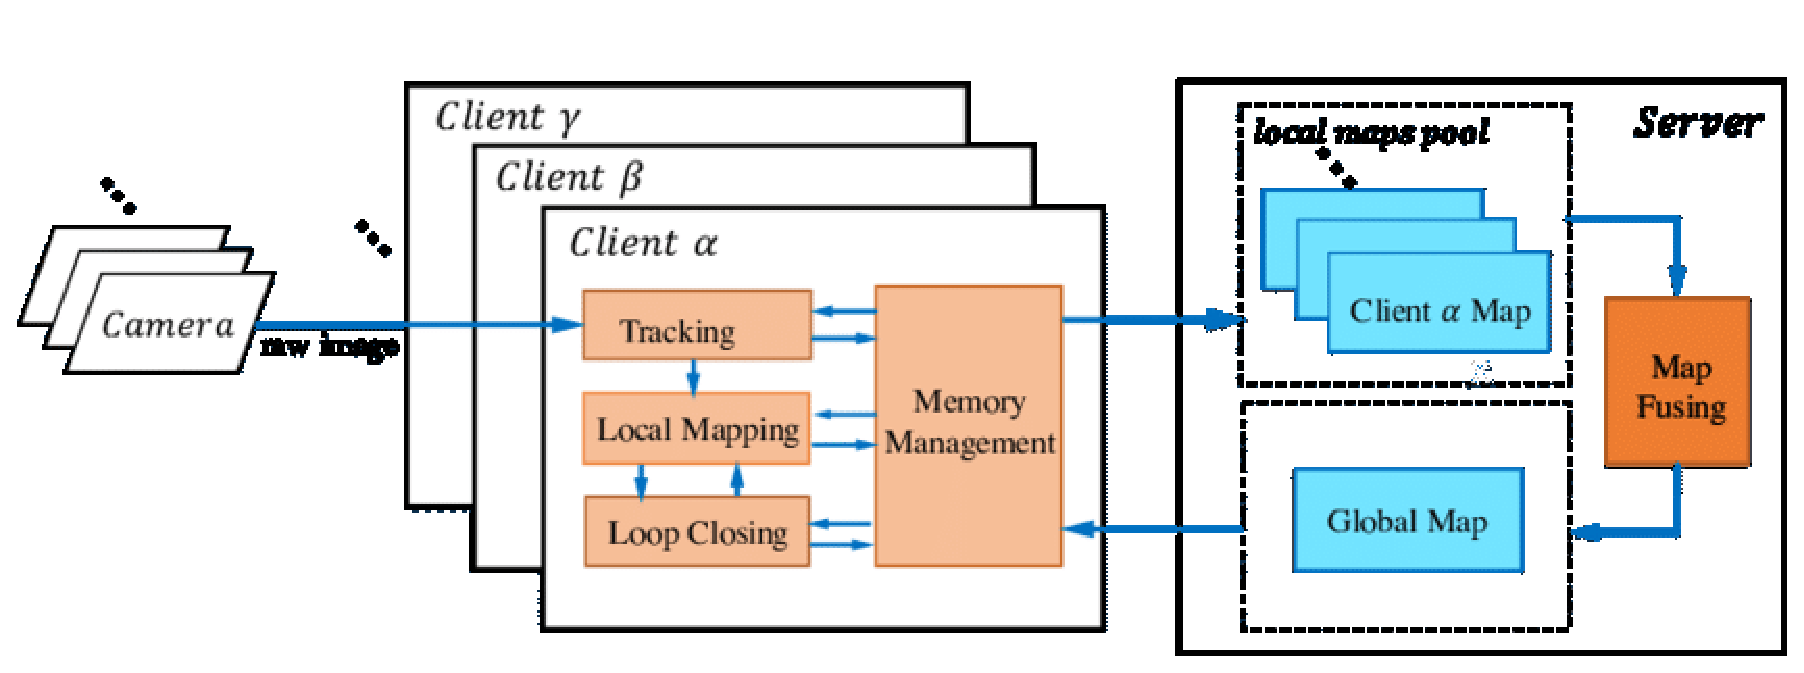
\includegraphics[width=5in]{Chapter2/CORBSLAMOverview.eps}
	\caption{The structure of CORB-SLAM system.}
	\label{fig:corbslamoverview} 
\end{figure}

\subsubsection{CORB-SLAM Client}
The robot-end client of CORB-SLAM is an ORB-SLAM client extended to have the functionality to communicate with the server, transmitting the local map information, with all functions and modules in original ORB-SLAM as listed in Chapter \ref{chp:orbslam} reserved.

\begin{figure}[H]
	\centering
	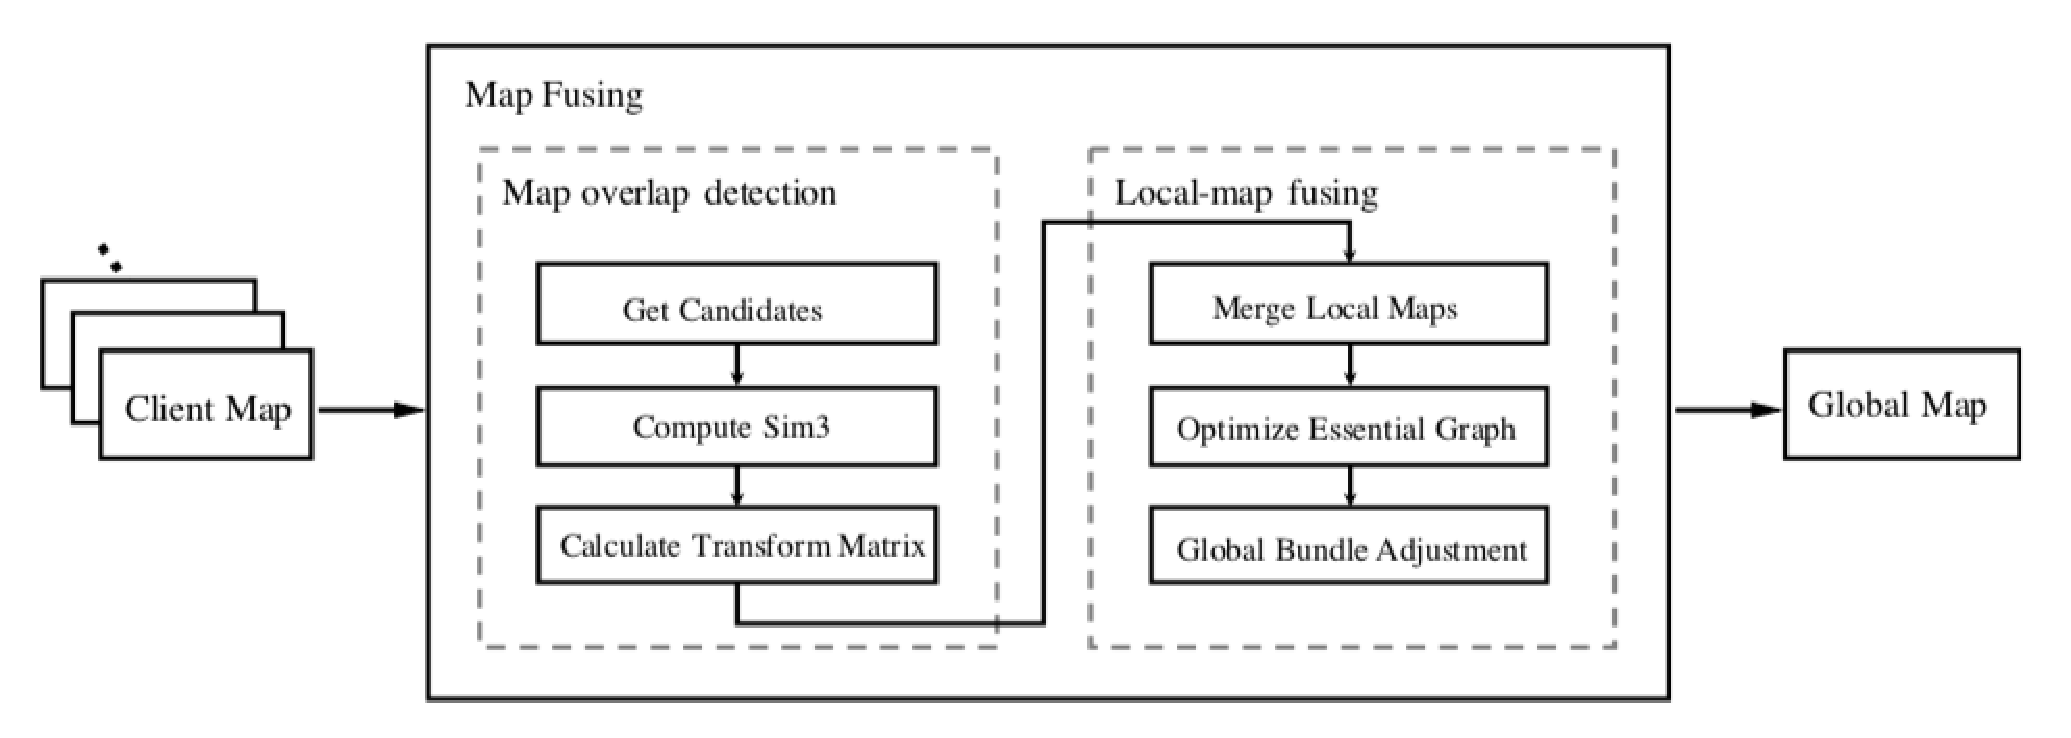
\includegraphics[width=5in]{Chapter2/corbslamserver.eps}
	\caption{The flowchart of Map Fusing module.}
	\label{fig:corbslamserver} 
\end{figure}

The server's map fusion module receives and fuses the clients ' local maps to achieve an optimized global map. Figure \ref{fig:corbslamserver} shows the map fusion algorithm, which includes three main parts: global map initialization, map overlap detection, as well as local map fusion.

\begin{enumerate}[1.]
	\item Global map initialization
	
	As the server system starts at the beginning, the server set the initial global map empty. As clients keep mapping and creating their local maps, the server receive data of local maps. After a first local map reaches the server, it will set as the initial global, based on which the global reference frame is decided.
	
	\item Map overlap detection
	
	To calculate relations between client maps, the server firstly detects the overlaps between local maps and then computes the transformation using Perspective-n-Point method.
	
	The map overlap detection module follows the same solution of ORB-SLAM2, which firstly extract keypoints from input images using ORB features, then compute similarities between images by distance between image descriptors based on Bag of Binary Words (DBoW3) approach.
	Then, after map overlaps are detected, RANSAC iterations are adopted to calculate the 7 degrees-of-freedom (DoF) transform matrix between the current keyframe and all rough candidates detected. With enough inliers, a similar candidata, $K_{\alpha}$ is optimized. If an enough number of inliers are calculated, the image overlap with $K_\alpha$ is accepted with the pose of $K_\alpha$, $T_{wc}$ calculate at the same time during optimization.
	
	\item Local map fusion 
	
	Local maps created by clients are merged into the consistent global map after an acceptable transform matrix has been obtained. Using Bundle Adjustment (BA), a global 7 DoF optimization is then performed to suppress map errors accumulated during the mapping process of each SLAM clients.
\end{enumerate}

After all process finished, the fused global map is resent to clients, and each client continues its own work to detect loop closure and correct loops on the received global map. If the global map is updated by computation on clients, the changes will be uploaded to server to update the map, and further transmitted to other clients by the server.

\section{Illumination Variance}

\subsection{Appearance Change From Illumination}

For vision systems concerned with locating in known environments, facing changes in appearance is an ongoing challenge. Changes in appearance can result from multiple sources, for example, 
\begin{inparaenum}[(i)]
	\item different lighting conditions,	
	\label{ls:appearancechange1}
	\item varying weather conditions, and
	\label{ls:appearancechange2}
	\item dynamic objects such as pedestrians or vehicles.
	\label{ls:appearancechange3}
\end{inparaenum}

During previous works by Colin McManus et al., they showed how to harness previous 3D structure knowledge, to suppress distracting objects, and how they are coped with by changing climate conditions, for an improved pose measurement in busy urban environments  \cite{churchill2012practice}. They proposed a new approach to addressing problem in \cite{maddern2014illumination} called the Illumination Variance Approach. 

Appearance change caused by different lighting conditions in (\ref{ls:appearancechange1}) is illustrated in Figure \ref{fig:shadecompare1} with pictures selected from St Lucia dataset \cite{glover2010fab}. Compared to approaches proposed in \cite{mcmanus2013distraction} and \cite{churchill2012practice}, illumination variance approach is not model-based, requiring less computational cost. And in most of applications of vSLAM, appearance changes caused by (\ref{ls:appearancechange1}) are a more common problem than (\ref{ls:appearancechange2}, \ref{ls:appearancechange3}). Therefore, how to combine illumination variance approach with multi-robot SLAM algorithms, One of the main aims focused on in this work is to improve the performance of location recognition modules in environments under changing lighting conditions.

\begin{figure}
	\centering
	\subfigure[pic1.]{
		\begin{minipage}[t]{0.4\linewidth}
			\centering
			\includegraphics[width=2in]{Chapter2/shadecompare1-0.eps}
			%\caption{fig1}
		\end{minipage}
	}
	\subfigure[pic2.]{
		\begin{minipage}[t]{0.4\linewidth}
			\centering
			\includegraphics[width=2in]{Chapter2/shadecompare1-1.eps}
			%\caption{fig2}
		\end{minipage}
	}
	\caption{Appearance changes caused by different lighting conditions. Pictures are selected from St Lucia dataset recording on 10/09/2009 8:45 am and 2:10 pm}
	\label{fig:shadecompare1}
\end{figure}

\subsection{Formulation}
Illumination variance approach proposed in \cite{maddern2014illumination}, is a simple method based on only one equation computing illumination variant images. The basic idea of this approach is to map color images to an illumination invariant color space, where illumination change caused by different lighting condition like shade can be suppressed. The mapping equation
is presented in Equation \ref{eq:iifinal}.

\begin{equation}
I=\log(R)-\alpha\log(G)-(1-\alpha)\log(B)
\label{eq:iifinal}
\end{equation}

Where, the raw image color channels are noted as $R, G, B$ and $I$ is the resulting invariant image illumination. As shown in \ref{eq:ii1}, $\alpha$ is a parameter that depends on each color channel's peak spectral responses ($ \lambda R, \lambda G, \lambda B$), normally obtainable in camera specifications. 

\begin{equation}
\frac{1}{\lambda_R}=\frac{\alpha}{\lambda_G}+\frac{1-\alpha}{\lambda_B}
\label{eq:ii1}
\end{equation}

Therefore, considering the peak spectral responses, $\alpha$ can be easily calculated as exposed in Equation \ref{eq:ii2}.

\begin{equation}
\alpha=\frac{(\frac{\lambda_B}{\lambda_G}-\frac{\lambda_B}{\lambda_R})}{(1-\frac{\lambda_B}{\lambda_R})}
\label{eq:ii2}
\end{equation}

the result images of illumination variance conversion are showed in Figure \ref{fig:iicompare1}.

\begin{figure}
	\centering
	\subfigure[pic1.]{
		\begin{minipage}[t]{0.4\linewidth}
			\centering
			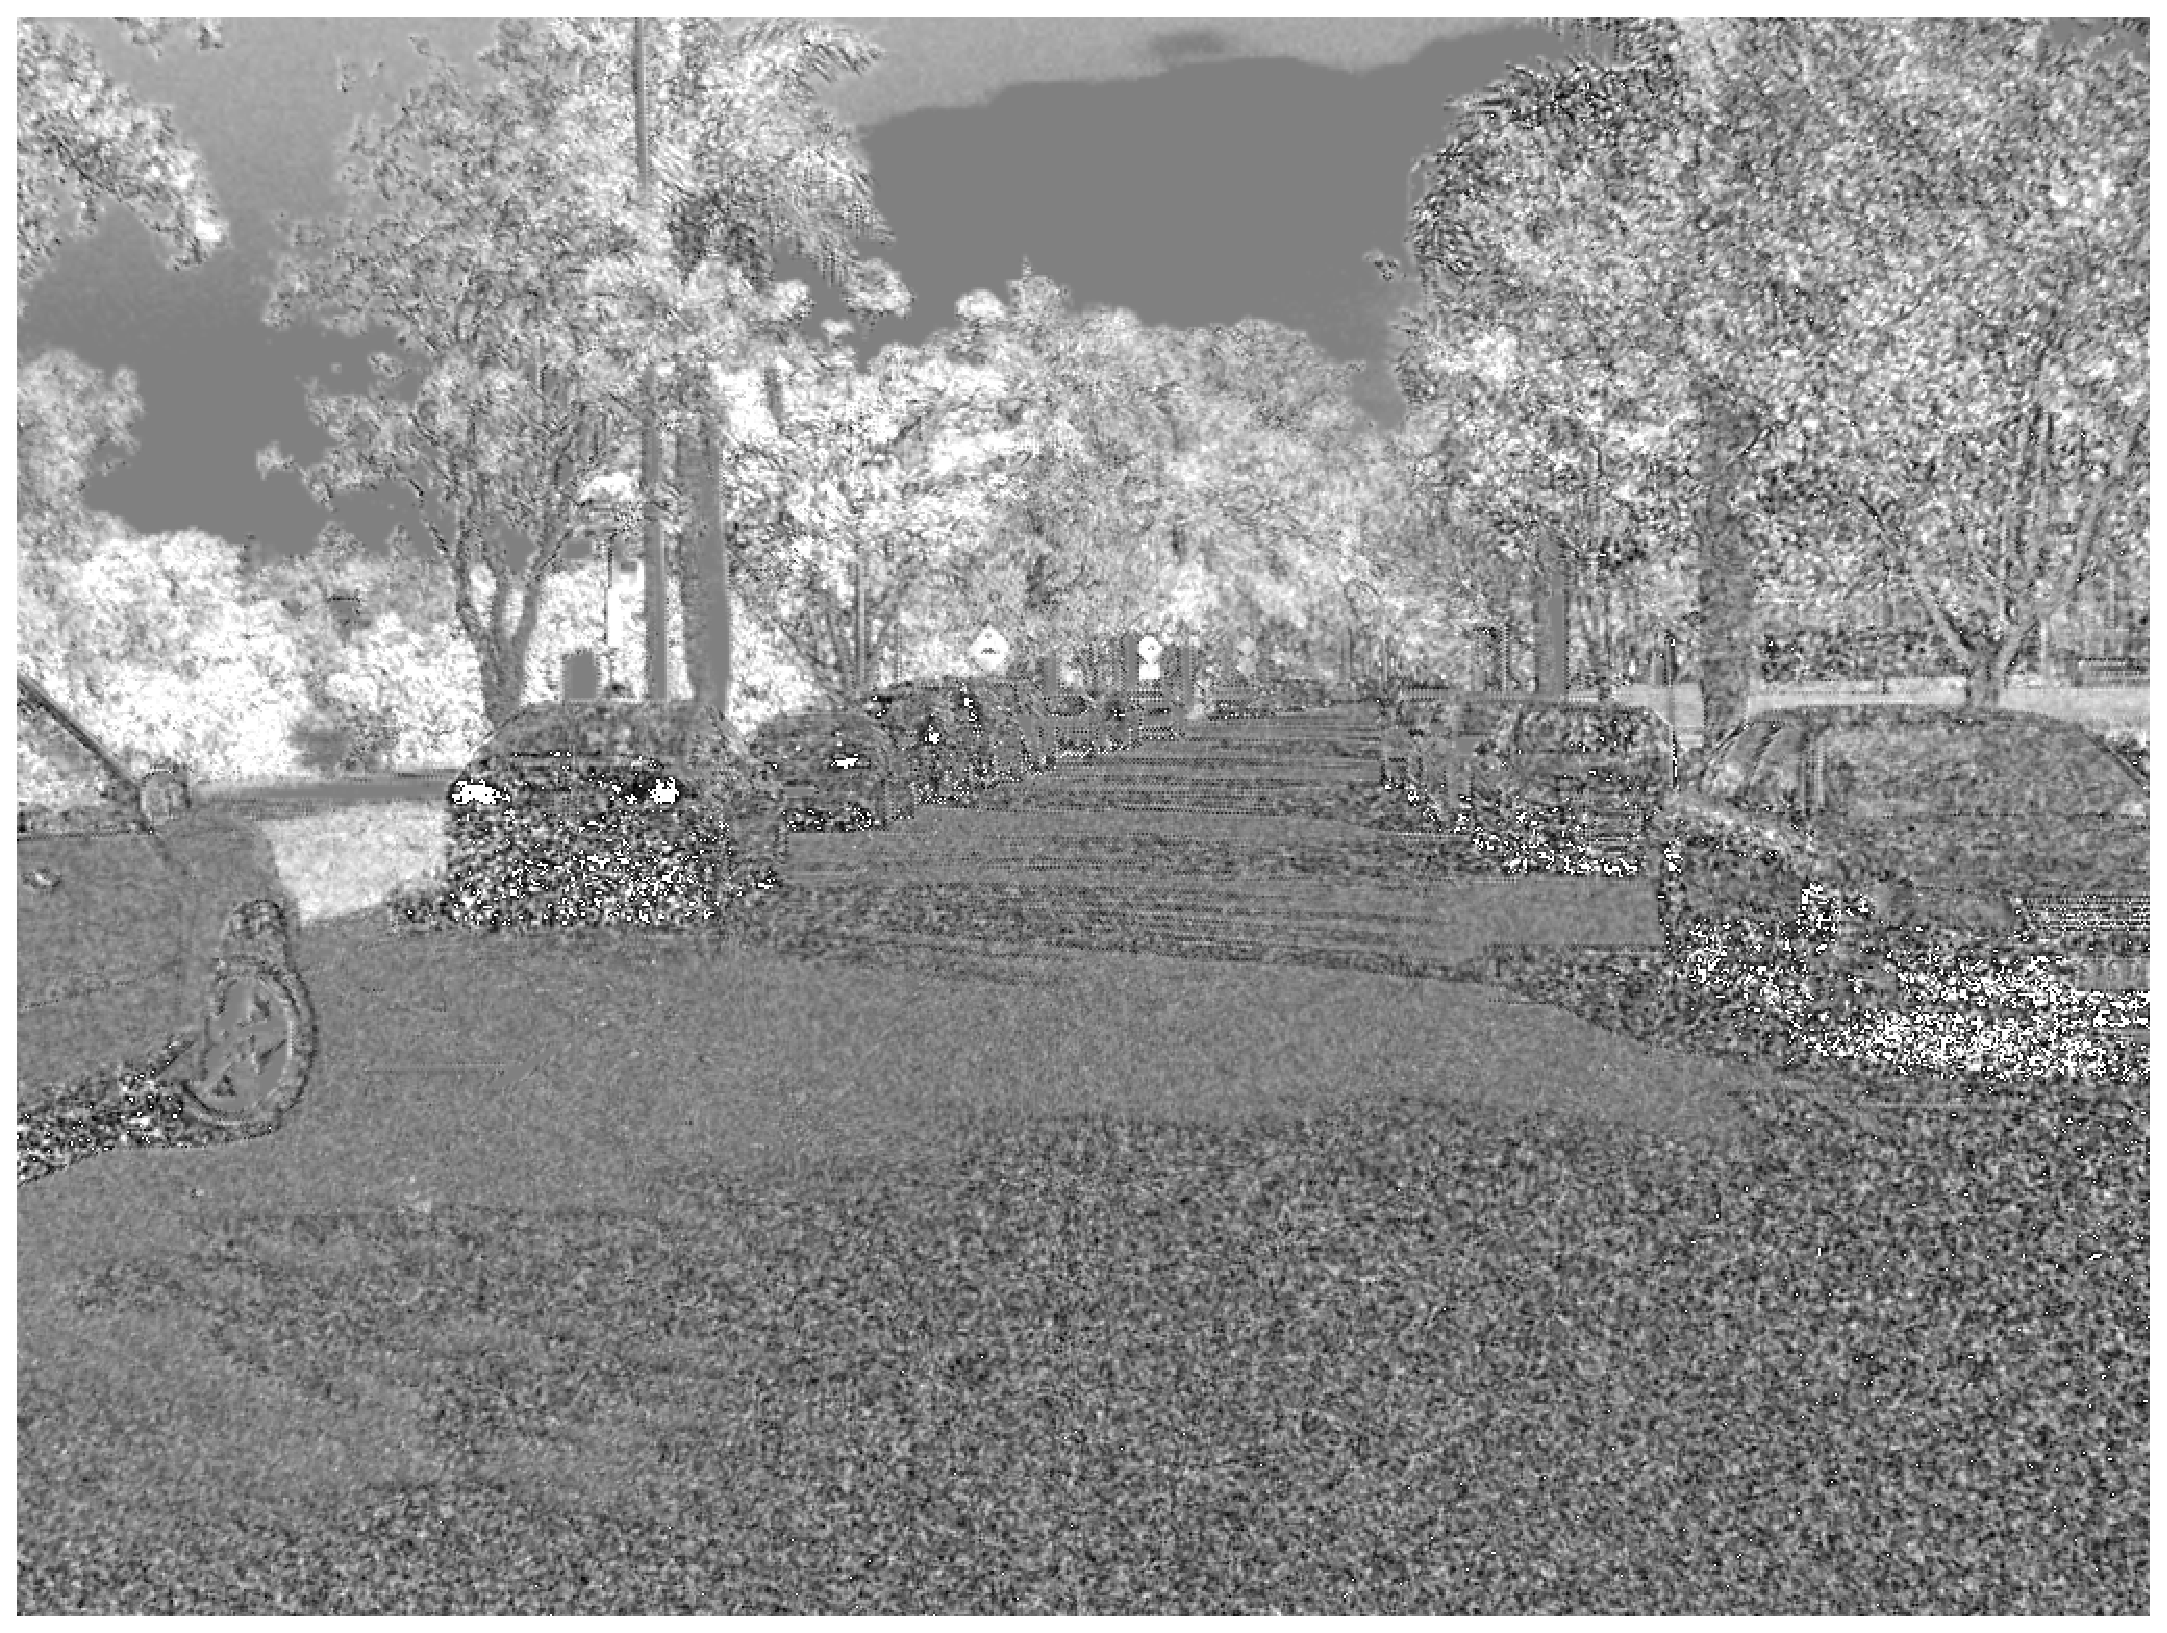
\includegraphics[width=2in]{Chapter2/iicompare1-0.eps}
			%\caption{fig1}
		\end{minipage}
	}
	\subfigure[pic2.]{
		\begin{minipage}[t]{0.4\linewidth}
			\centering
			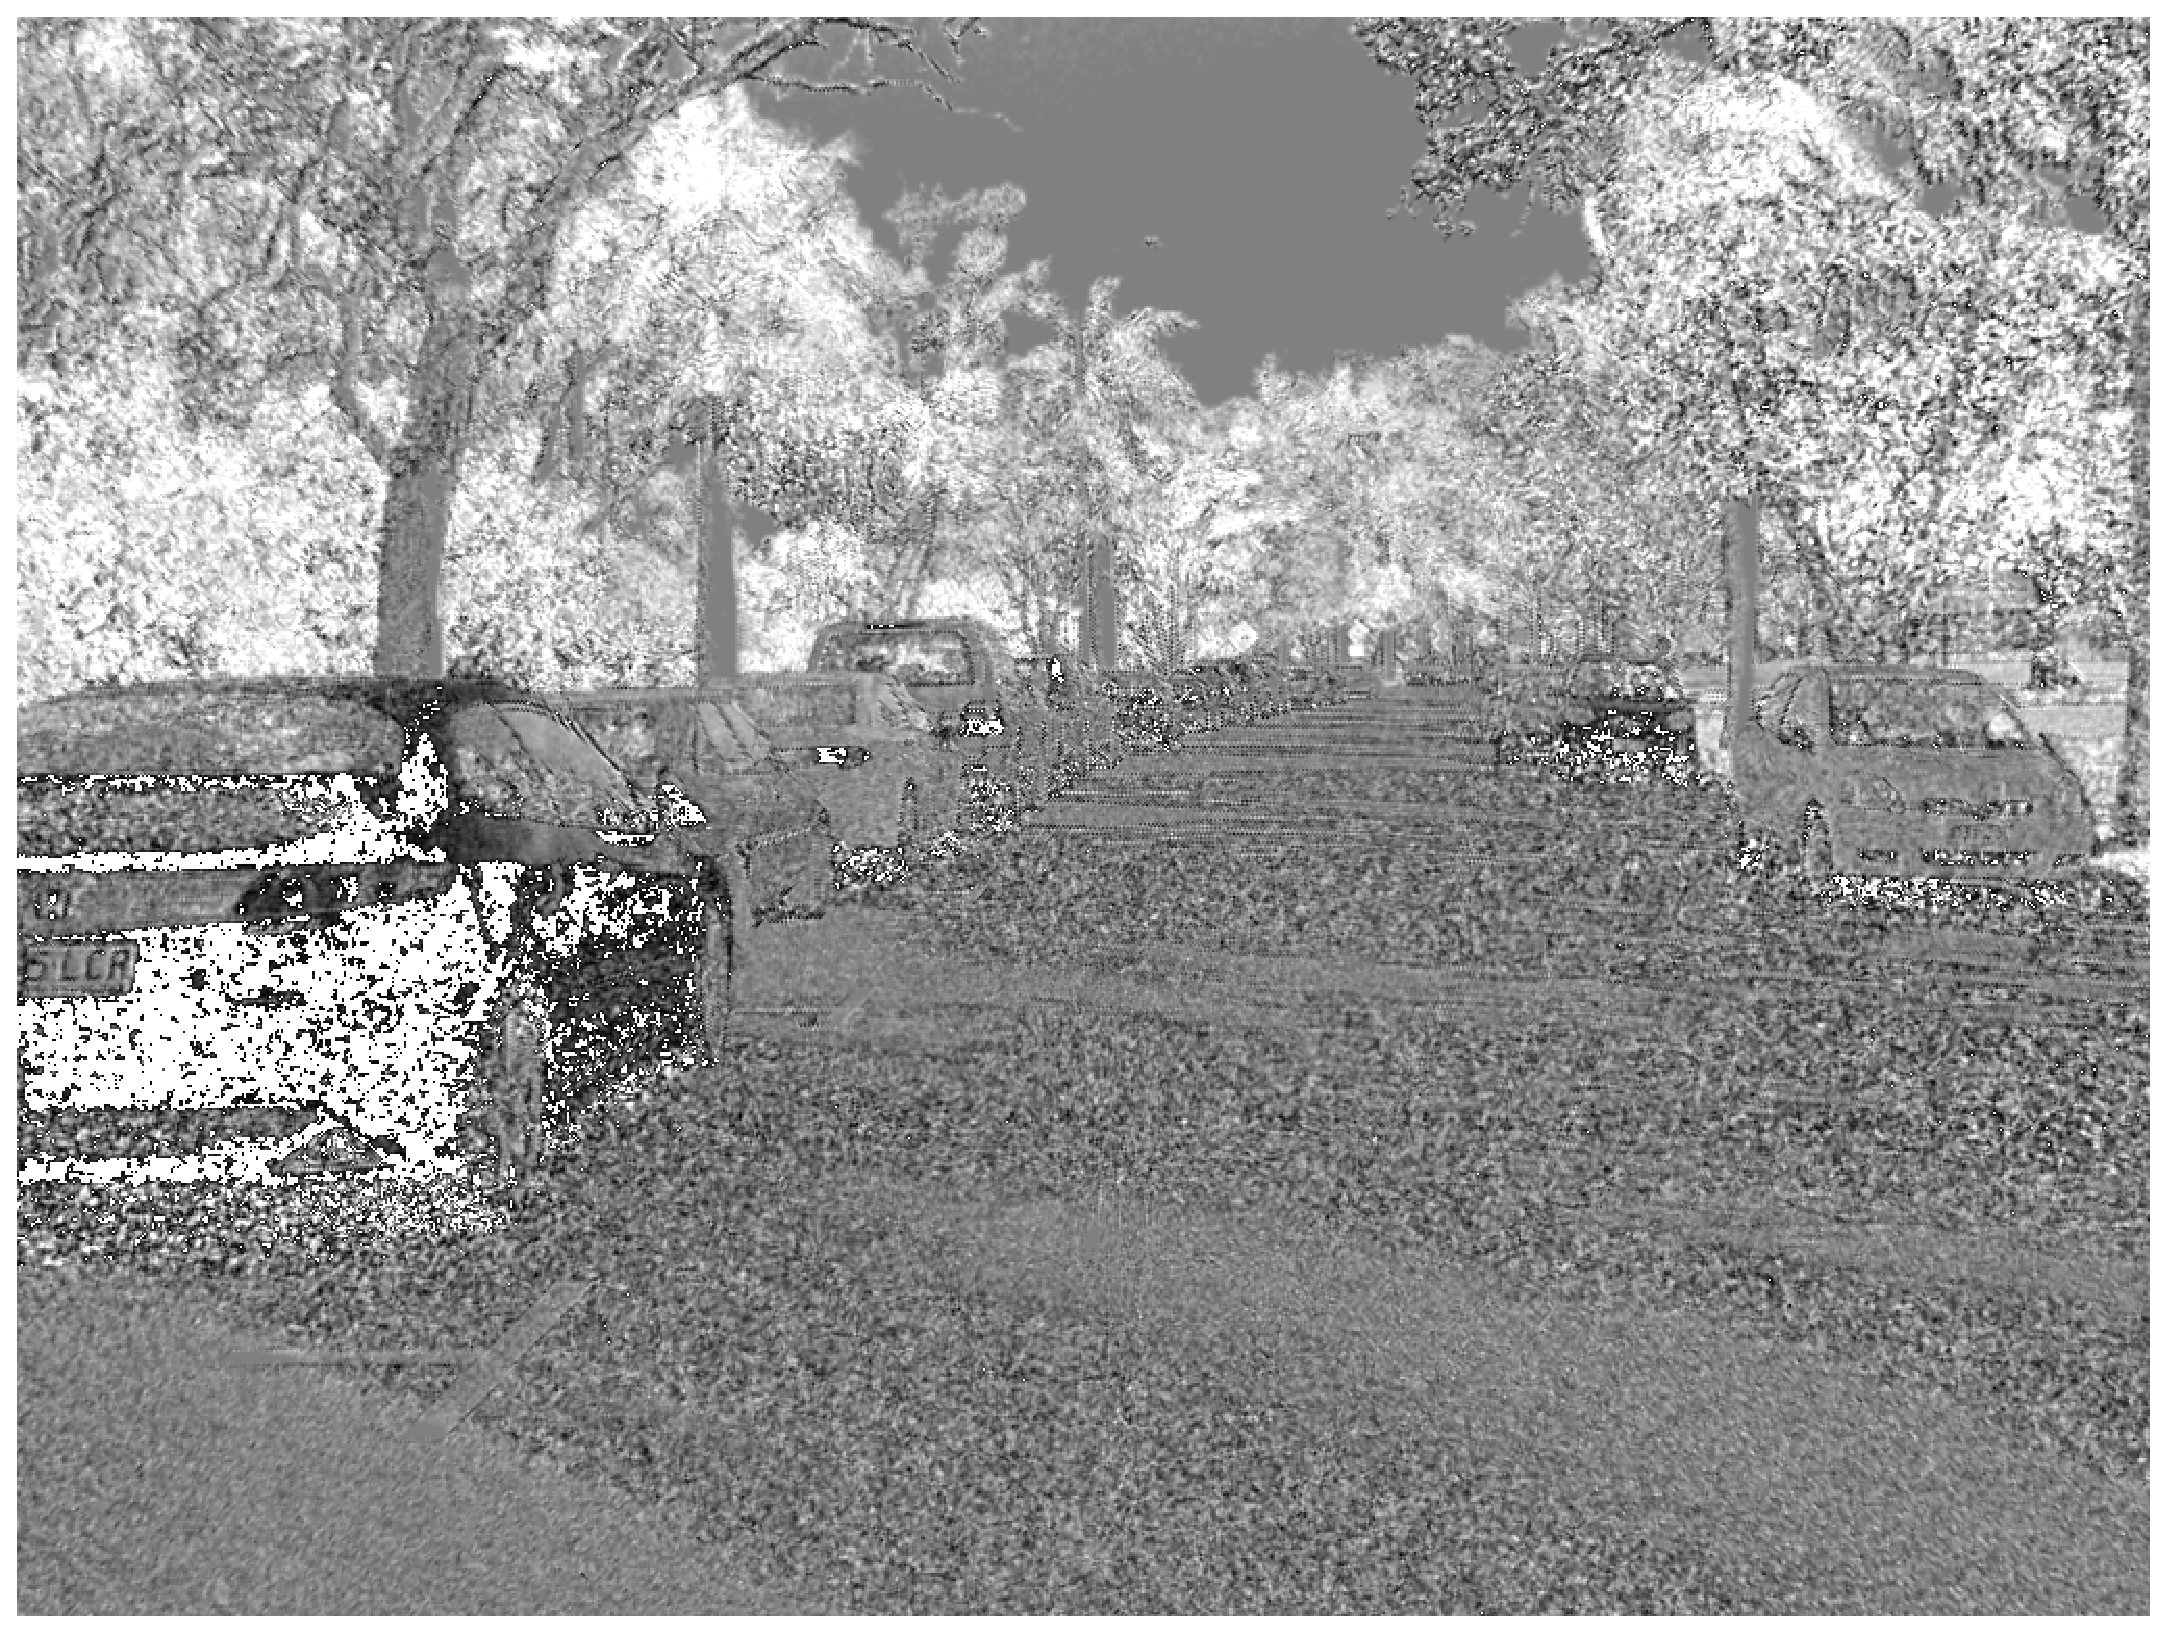
\includegraphics[width=2in]{Chapter2/iicompare1-1.eps}
			%\caption{fig2}
		\end{minipage}
	}
	\caption{Illumination invariance result images in St Lucia dataset. It shows how this approach suppress the effects caused by sun}
	\label{fig:iicompare1}
\end{figure}

\subsection{Application of Localization}
An open source toolbox called OpenABLE is implemented in \cite{arroyo2016openable} for lifelong visual localization. The proposed implementation in \cite{arroyo2016openable} uses the philosophy of the topological location recognition approach called ABLE introduced in \cite{arroyo2014bidirectional, arroyo2014fast, arroyo2015towards} using illumination variant images for relocation. 

A graphic representation about how the methodology proposed by OpenABLE is showed in Figure \ref{fig:openableoverview}.

\begin{figure}[H]
	\centering
	\includegraphics[width=5in]{Chapter2/OPENABLEOverview.eps}
	\caption{A graphic demonstration about how ABLE works.}
	\label{fig:openableoverview} 
\end{figure}

The limitation of illumination variance approach is the transformation process produces resultant images with low resolution because all pixel values are turned into log values. These low-resolution resultant images still can be used as the input images of visual topological localization where high resolution images are actually not needed. But in the mapping task, illumination variant images are too blurry to estimate camera motion and then reconstruct the map. Therefore, to improve the mapping performance in changing illumination conditions, rgb images and illumination variant images are both needed to perform relocalization and mapping, as the block-flow proposed in \cite{mcmanus2014shady} presented in \ref{fig:iioverview}.

\begin{figure}[H]
	\centering
	\includegraphics[width=5in]{Chapter2/COISLAMOverview.eps}
	\caption{Block-flow diagram of the combined stereo localisation approach.}
	\label{fig:iioverview} 
\end{figure}

In the framework presented in \ref{fig:iicompare1}, there is a second localizer making use of illumination invariant images in parallel with the main localization system. In \cite{maddern2014illumination}, although the metric relative poses calculated from illumination variant images tends wo be more noisy, the integrated localizer are less likely to fail if the scene appearance change is due to sunlight intensity direction or spectrum variation.

%=== END OF CHAPTER TWO ===
\newpage

%=== CHAPTER THREE (3) ===
%=== (Actual work done and contribution, including literature survey) ===

\chapter{Approach (Actual work done and contribution, including literature survey)}

\section{Evaluation of CORBSLAM}

\section{Modification to CORBSLAM}

\section{CORBSLAM with Illumination Variance}




%=== END OF CHAPTER THREE ===
\newpage

%=== CHAPTER FOUR (4) ===
%=== Test and Experiments ===

\chapter{Test and Experiments}

\section{Datasets}

Evaluation are performed in several datasets including KITTI Visual Odometry 2012 dataset\cite{Geiger2012CVPR},  Oxford RobotCar dataset\cite{maddern20171} and NTU dataset collected in NTU. The listing of used datasets is shown in Table \ref{tbl:datasetsinfo}


\begin{table*}
	\centering
	\caption{Information of datasets used }
	\begin{tabular}{|c|c|c|c|}
		\hline
		Datasets & Settings & Approx Scale & Diversity \\
		\hline
		KITTI &  rural area & $<$ 1 hour & one city, one weather condition, daytime \\
		\hline
		Oxford &  city & 214 hours & one city, multiple weather conditions, daytime \\
		\hline
		NTU &  campus & $<$ 1 hour & one campus (NTU), one weather condition \\
		\hline
	\end{tabular}
	\label{tbl:datasetsinfo}
\end{table*}

\subsection{KITTI Visual Odometry Dataset}

KITTI Visual Odometry 2012 is part of the \cite{Geiger2012CVPR, Menze2015CVPR} KITTI Vision Benchmarck Suite. KITTI data sets are captured by driving around a city of medium size, in rural areas and on highways. The recording platform is equipped with two stereo camera systems of high resolution capturing color and gray images, a Velodyne HDL-64E LIDAR and an OXTS RT 3003 localization system combining GPS, GLONASS, IMU and RTK correction signals. 

KITTI Visual Odometry Evaluation 2012 provides 11 sequences with ground truth trajectories for training, and another 11 sequences without ground truth for evaluation. Example images are shown in Figure \ref{fig:kittiexamples}. 

\begin{figure}[H]
	\centering
	\includegraphics[width=5in]{Chapter4/kittiexamples.eps}
	\caption{Example image in KITTI Visual Odometry 2012 dataset.}
	\label{fig:kittiexamples} 
\end{figure}

\subsection{Oxford RobotCar Dataset}
Oxford RobotCar Dataset is presented by Will Maddern et al. in \cite{maddern20171}, as a challenging dataset for autonomous driving. Collected over the period of May 2014 to December 2015, this datasets recorded images from 6 cameras mounted Nissan LEAF, along with LIDAR, GPS and INS ground truth. Images were recorded under different weather and illumination condition  from 9:00 to 16:00 on average, from May to December. Example images is shown in Figure \ref{fig:robotcarexamples}.

\begin{figure}[H]
	\centering
	\includegraphics[width=5in]{Chapter4/robotcarexamples.eps}
	\caption{Example image in robotcar dataset.}
	\label{fig:robotcarexamples} 
\end{figure}

The RobotCar platform is a Nissan LEAF equipped with sensors as following \cite{maddern20171}:

\begin{enumerate}
	\item Stereo Camera: Bumblebee XB3 trinocular stereo camera $\times$ 1, 1/3'' Sony ICX445 CCD, 1280$\times$960$\times$3, 16Hz, 3.88mm lens, $66^{\circ}$ HFoV, 12/24cm baseline, global shutter.
	\item Monocular Camera: Grasshopper2 $\times$ 3, 2/3'' ICX285 CCD, 1024$\times$1024, 11.1Hz, 2.67mm fisheye lens, $180^{\circ}$, global shutter.
	\item 2D LIDARL SICK LMS-151 2D LIDAR $\times$ 2, $270^{\circ}$ FoV, 50Hz, 50m range, $0.5^{\circ}$ resolution.
	\item 3D LIDAR: SICK LD-MRS 3D LIDAR $\times$ 1, $85^{\circ}$ HFoC, $3.2^{\circ}$ VFoV, 4 panes, 12.5Hz, 50m range, $0.125^{\circ}$ resolution.
	\item GPS/INS Module: NovAtel SPAN-CPT ALIGN inertial and GPS navigation system $\times$ 1, 6 axis, 50Hz, GPS/GLONASS, dual antenna.
 \end{enumerate}

The RobotCar platform and the sensor locations are demonstrated in Figure \ref{fig:robotcarsensorlocation}.

\begin{figure}[H]
	\centering
	\includegraphics[width=5in]{Chapter4/robotcarsensorlocation.eps}
	\caption{The robotcar platform and sensor location diagram.}
	\label{fig:robotcarsensorlocation} 
\end{figure}

RobotCar dataset is especially suitable to evaluate long-term SLAM systems, since it contains images taken in different hours of daytime under different illumination conditions, and in different seasons. The comparison between image in different illumination conditions and different seasons is shown in Figure \ref{fig:robotcarcomparisonseason}.

\begin{figure}
	\centering
	\subfigure[Image captured in 14:49 07/14/2014.]{
		\label{sfig:robotcarjulyraw}
		\begin{minipage}[t]{0.4\linewidth}
			\centering
			\includegraphics[width=2in]{Chapter4/robotcarfeb.eps}
			%\caption{fig1}
		\end{minipage}
	}
	\subfigure[Image captured in 12:32 02/24/2015.]{
	\label{sfig:robotcarfebraw}
		\begin{minipage}[t]{0.4\linewidth}
			\centering
			\includegraphics[width=2in]{Chapter4/robotcardec.eps}
			%\caption{fig2}
		\end{minipage}
	}
	\caption{Comparison of images captured in the same location in different seasons in RobotCar dataset.}
	\label{fig:robotcarcomparisonseason}
\end{figure}
	
\subsection{NTU Dataset}
\label{sec:ntuinfo}
Our NTU dataset \cite{zhang2018two} is collected by multi ground robots consisting of two husky UGV platforms, recording driving around the carpark in front of School of EEE building.

Our UGV platform is a HUSKY Clearpath robot, equipped with a ZED stereo camera $\times$ 1, 672$\times$376, $87^{\circ}$ HFoV, $56^{\circ}$ VFoV. The picture of the platform and example images are shown in Figure \ref{fig:ntuugvplatform} and \ref{fig:ntuexamples}.

%The UAV platform is assembled with: PIXRACER V1.0 AUTOPILOT Controller Module, DJI E Series 620S Motor Package, a uBLOXNEO-M8N GPS Module and a monocular camera mounted at a depression angle of 20 degree. The overview picture of the UAV is shown in Figure \ref{fig:ntuuavplatform}

The dataset provides 4 rosbag files. 3 of them are recorded by UGV, while the other one is recorded by UAV. The basic information of 4 rosbags are listed in Table \ref{tbl:ntubagsinfo}. And the ground truth trajectories are shown in Figure \ref{fig:ntugt}.

\begin{figure}
	\centering
	\subfigure[Ground truth trajectory of Bag.0.]{
		\begin{minipage}[t]{0.4\linewidth}
			\centering
			\includegraphics[width=2in]{Chapter4/NTU/0446/plots/trajectory_top_gt_sim3_-1.pdf}
			%\caption{fig1}
		\end{minipage}
	}
	\subfigure[Ground truth trajectory of Bag.1.]{
		\begin{minipage}[t]{0.4\linewidth}
			\centering
			\includegraphics[width=2in]{Chapter4/NTU/0454/plots/trajectory_top_gt_sim3_-1.pdf}
			%\caption{fig2}
		\end{minipage}
	}
%	\vfill
%		\subfigure[Ground truth trajectory of Bag.2.]{
%		\begin{minipage}[t]{0.4\linewidth}
%			\centering
%			\includegraphics[width=2in]{Chapter4/NTU/UGV/plots/trajectory_top_gt_sim3_-1.pdf}
%			%\caption{fig1}
%		\end{minipage}
%	}
%	\subfigure[Ground truth trajectory of Bag.3.]{
%		\begin{minipage}[t]{0.4\linewidth}
%			\centering
%			\includegraphics[width=2in]{thereisafigure.eps}
%			%\caption{fig2}
%		\end{minipage}
%	}
	\caption{Ground truth information of each rosbags in NTU Dataset.}
	\label{fig:ntugt}
\end{figure}

\begin{table*}
	\centering
	\caption{Main characteristics of the rosbags in NTU Dataset used in the experiment.}
	\begin{tabular}{|c|c|c|c|c|}
		\hline
		Bag No. & Data(M/D/Y)  & Platform & Height(m) & Dep. Angle  \\
		\hline
		0&10/27/2018& UGV & $\approx 0.7m$ & $0^\circ$ \\
		\hline
		1&10/27/2018& UGV & $\approx 0.7m$ & $0^\circ$ \\
		\hline
%		2&03/08/2019& UGV & $\approx 0.7m$ & $0^\circ$ \\
%		\hline
%		3&03/08/2019& UAV & $\approx 2m$ & $20^\circ$ \\
%		\hline
	\end{tabular}
	\label{tbl:ntubagsinfo}
\end{table*}

\begin{figure}[H]
	\centering
	\includegraphics[width=5in]{Chapter4/ntuhuskytugv.eps}
	\caption{Overview picture of NTU Husky platform.}
	\label{fig:ntuugvplatform} 
\end{figure}

%\begin{figure}[H]
%	\centering
%	\includegraphics[width=5in]{Chapter4/ntuuav0.eps}
%	\caption{Overview picture of NTU Husky platform.}
%	\label{fig:ntuuavplatform} 
%\end{figure}

\begin{figure}[H]
	\centering
	\includegraphics[width=5in]{Chapter4/ntuexamples.eps}
	\caption{Example images of NTU dataset.}
	\label{fig:ntuexamples} 
\end{figure}

\section{Evaluation of CORBSLAM}

\ifoutputscaleerror
\subsection{Evaluation on multi ground robots}
\fi

\subsection{KITTI Datasets}
\label{sec:kittievaluate}
In order to evaluate CORB-SLAM system, sequence 00 is utilized and separated into two sub sequences with proper length of overlap. The following separating method is employed: We assume the time period of a KITTI sequence if $Seq.0[0,t]$. Then the sequence is separated into two sub sequences $Seq.01[0,\frac{t}{2}+\delta{t}]$ and $Seq.02[\frac{t}{2},t]$ as the assumed input of two client robots. 

Therefore, in this case, Sequence 00 containing $f=4541frames$ and covering a total distance of $s=1856m$ is separated into two partial sequences: Seq.0$[0, \frac{2}{3}f]$ and Seq.1$[\frac{1}{3}f, f]$, both containing  $\frac{2}{3}f\approx{3027frames}$ and covering distances of $\frac{2}{3}s\approx{1237m}$ (a rough estimate since distances between each pair of frames are not equal). 

The ground truth information of Seq.0, Seq.1 and the complete ground truth trajectory of Sequence 00 are shown for reference in Figure \ref{fig:kittigt}. And Figure \ref{fig:kittiresults} demonstrates mapping results of each partial sequence and the map fusion results of the server. Four charts in Figure \ref{fig:kittiquanresult} contains quantitative evaluation results, with corresponding numeric results shown in Table \ref{tbl:ntuquanresult}.

Clients' quantitative mapping results of each partial sequence are provided in Figure \ref{fig:kittiseq0quanresult}, \ref{fig:kittiseq1quanresult}  and Table \ref{tbl:kittiseq0quanresult}, \ref{tbl:kittiseq1quanresult}. And because the two partial sequences are extracted from Sequence 00, so the completed mapping results of CORB-SLAM client on Sequence 00 can be provided as a comparison by Figure \ref{fig:kittientirequanresult}, \ref{fig:kitticlientmapping} and Table \ref{tbl:kitticlientquanresult} in the same format as above. Results are further discussed in Section \ref{sec:disussmultiground}.


\begin{figure}
	\centering
	\subfigure[Ground truth trajectory of Seq.0.]{
		\begin{minipage}[t]{0.4\linewidth}
			\centering
			\includegraphics[width=2in]{Chapter4/KITTI/00server/32/plots/trajectory_side_gt_sim3_-1.pdf}
			%\caption{fig1}
		\end{minipage}
	}
	\subfigure[Ground truth trajectory of Seq.1.]{
		\begin{minipage}[t]{0.4\linewidth}
			\centering
			\includegraphics[width=2in]{Chapter4/KITTI/00server/33/plots/trajectory_side_gt_sim3_-1.pdf}
			%\caption{fig2}
		\end{minipage}
	}
	\vfill
	\subfigure[Ground truth trajectory of complete Sequence 00.]{
		\begin{minipage}[t]{\linewidth}
			\centering
			\includegraphics[width=5in]{Chapter4/KITTI/00server/plots/trajectory_side_gt_sim3_-1.pdf}
			%\caption{fig1}
		\end{minipage}
	}
	\caption{Ground truth trajectory of partial and complete sequences of KITTI Datasets.}
	\label{fig:kittigt}
\end{figure}

\begin{figure}
	\centering
	\subfigure[Relative translation error.]{
		\begin{minipage}[t]{0.4\linewidth}
			\centering
			\includegraphics[width=2in]{Chapter4/KITTI/00/gps/plots/rel_translation_error.pdf}
			%\caption{fig1}
		\end{minipage}
	}
	\subfigure[Relative translation error by percent.]{
		\begin{minipage}[t]{0.4\linewidth}
			\centering
			\includegraphics[width=2in]{Chapter4/KITTI/00/gps/plots/rel_translation_error_perc.pdf}
			%\caption{fig2}
		\end{minipage}
	}
	\vfill
	\subfigure[Relative yaw error.]{
		\begin{minipage}[t]{0.4\linewidth}
			\centering
			\includegraphics[width=2in]{Chapter4/KITTI/00/gps/plots/rel_yaw_error.pdf}
			%\caption{fig1}
		\end{minipage}
	}
\ifoutputscaleerror
	\subfigure[Scale error.]{
		\begin{minipage}[t]{0.4\linewidth}
			\centering
			\includegraphics[width=2in]{Chapter4/KITTI/00/gps/plots/scale_error_sim3_-1.pdf}
			%\caption{fig2}
		\end{minipage}
	}
\fi
	\caption{Quantitative evaluation results of CORB-SLAM client mapping the entire KITTI Sequence 00.}
	\label{fig:kittientirequanresult}
\end{figure}

\begin{figure}
	\centering
	\subfigure[Relative translation error.]{
		\begin{minipage}[t]{0.4\linewidth}
			\centering
			\includegraphics[width=2in]{Chapter4/KITTI/00server/32/plots/rel_translation_error.pdf}
			%\caption{fig1}
		\end{minipage}
	}
	\subfigure[Relative translation error by percent.]{
		\begin{minipage}[t]{0.4\linewidth}
			\centering
			\includegraphics[width=2in]{Chapter4/KITTI/00server/32/plots/rel_translation_error_perc.pdf}
			%\caption{fig2}
		\end{minipage}
	}
	\vfill
	\subfigure[Relative yaw error.]{
		\begin{minipage}[t]{0.4\linewidth}
			\centering
			\includegraphics[width=2in]{Chapter4/KITTI/00server/32/plots/rel_yaw_error.pdf}
			%\caption{fig1}
		\end{minipage}
	}
\ifoutputscaleerror
	\subfigure[Scale error.]{
		\begin{minipage}[t]{0.4\linewidth}
			\centering
			\includegraphics[width=2in]{Chapter4/KITTI/00server/32/plots/scale_error_sim3_-1.pdf}
			%\caption{fig2}
		\end{minipage}
	}
\fi
	\caption{Quantitative evaluation results of CORB-SLAM client mapping  KITTI partial Seq.0.}
	\label{fig:kittiseq0quanresult}
\end{figure}

\begin{figure}
	\centering
	\subfigure[Relative translation error.]{
		\begin{minipage}[t]{0.4\linewidth}
			\centering
			\includegraphics[width=2in]{Chapter4/KITTI/00server/33/plots/rel_translation_error.pdf}
			%\caption{fig1}
		\end{minipage}
	}
	\subfigure[Relative translation error by percent.]{
		\begin{minipage}[t]{0.4\linewidth}
			\centering
			\includegraphics[width=2in]{Chapter4/KITTI/00server/33/plots/rel_translation_error_perc.pdf}
			%\caption{fig2}
		\end{minipage}
	}
	\vfill
	\subfigure[Relative yaw error.]{
		\begin{minipage}[t]{0.4\linewidth}
			\centering
			\includegraphics[width=2in]{Chapter4/KITTI/00server/33/plots/rel_yaw_error.pdf}
			%\caption{fig1}
		\end{minipage}
	}
\ifoutputscaleerror
	\subfigure[Scale error.]{
		\begin{minipage}[t]{0.4\linewidth}
			\centering
			\includegraphics[width=2in]{Chapter4/KITTI/00server/33/plots/scale_error_sim3_-1.pdf}
			%\caption{fig2}
		\end{minipage}
	}
\fi
	\caption{Quantitative evaluation results of CORB-SLAM client mapping  KITTI partial Seq.1.}
	\label{fig:kittiseq1quanresult}
\end{figure}

\begin{table*}
	\centering
	\caption{Quantitative results of mapping unseparated Sequence 00.}
	\begin{threeparttable}
			\ifoutputscaleerror
		\begin{tabular}{|c|c|c|c|c|}
			\hline
			Distance(m)\tnote{1} & Rel. Trans.(m)\tnote{2}  & Rel. Trans.($\%$)\tnote{3} & Rel. Yaw(deg)\tnote{4} & Scale Err.($\%$)\tnote{5}  \\
			\hline
			371& 229.69 & 61.91 & 0.37 & - \\
			\hline
			742&260.10& 35.05 & 0.37 & - \\
			\hline
			1113&260.20& 23.38 & 0.31 & - \\
			\hline
			1485&240.93& 16.22 & 0.40 & - \\
			\hline
			1856&255.16& 13.74 & 0.32 & 0.05\\
			\hline
		\end{tabular}
		\begin{tablenotes}
			\footnotesize
			\item[1] Distance in meter traveled before each time of statistics. 
			\item[2] Mean relative translation error in meter.
			\item[3] Mean relative translation error in percent.
			\item[4] Mean relative yaw error in degree.
			\item[5] Median scale error in percent.
		\end{tablenotes}
	\fi
	
			\begin{tabular}{|c|c|c|c|c|}
		\hline
		Distance(m)\tnote{1} & Rel. Trans.(m)\tnote{2}  & Rel. Trans.($\%$)\tnote{3} & Rel. Yaw(deg)\tnote{4}   \\
		\hline
		371& 229.69 & 61.91 & 0.37  \\
		\hline
		742&260.10& 35.05 & 0.37 \\
		\hline
		1113&260.20& 23.38 & 0.31  \\
		\hline
		1485&240.93& 16.22 & 0.40 \\
		\hline
		1856&255.16& 13.74 & 0.32 \\
		\hline
	\end{tabular}
	\begin{tablenotes}
		\footnotesize
		\item[1] Distance in meter traveled before each time of statistics. 
		\item[2] Mean relative translation error in meter.
		\item[3] Mean relative translation error in percent.
		\item[4] Mean relative yaw error in degree.
	\end{tablenotes}
	\end{threeparttable}
	\label{tbl:kitticlientquanresult}
\end{table*}

\begin{table*}
	\centering
	\caption{Quantitative results of mapping Seq.0.}
	\begin{threeparttable}
		\begin{tabular}{|c|c|c|c|c|}
			\hline
			Distance(m)\tnote{1} & Rel. Trans.(m)\tnote{2}  & Rel. Trans.($\%$)\tnote{3} & Rel. Yaw(deg)\tnote{4}   \\
			\hline
			229& 161.01 & 70.31 & 0.40  \\
			\hline
			458&267.43& 58.38 & 0.42\\
			\hline
			688&299.07& 43.47 & 0.31 \\
			\hline
			917&306.37& 33.41 & 0.39 \\
			\hline
			1146&256.09& 22.35 & 0.34 \\
			\hline
		\end{tabular}
		\begin{tablenotes}
			\footnotesize
			\item[1] Distance in meter traveled before each time of statistics. 
			\item[2] Mean relative translation error in meter.
			\item[3] Mean relative translation error in percent.
			\item[4] Mean relative yaw error in degree.
		\end{tablenotes}
	
	\ifoutputscaleerror
			\begin{tabular}{|c|c|c|c|c|}
		\hline
		Distance(m)\tnote{1} & Rel. Trans.(m)\tnote{2}  & Rel. Trans.($\%$)\tnote{3} & Rel. Yaw(deg)\tnote{4} & Scale Err.($\%$)\tnote{5}  \\
		\hline
		229& 161.01 & 70.31 & 0.40 & - \\
		\hline
		458&267.43& 58.38 & 0.42& - \\
		\hline
		688&299.07& 43.47 & 0.31 & - \\
		\hline
		917&306.37& 33.41 & 0.39& - \\
		\hline
		1146&256.09& 22.35 & 0.34 & $2.47\times10^{-3}$\\
		\hline
	\end{tabular}
	\begin{tablenotes}
		\footnotesize
		\item[1] Distance in meter traveled before each time of statistics. 
		\item[2] Mean relative translation error in meter.
		\item[3] Mean relative translation error in percent.
		\item[4] Mean relative yaw error in degree.
		\item[5] Median scale error in percent.
	\end{tablenotes}
\fi
	\end{threeparttable}
	\label{tbl:kittiseq0quanresult}
\end{table*}

\begin{table*}
	\centering
	\caption{Quantitative results of mapping Seq.1.}
	\begin{threeparttable}
		\begin{tabular}{|c|c|c|c|c|}
			\hline
			Distance(m)\tnote{1} & Rel. Trans.(m)\tnote{2}  & Rel. Trans.($\%$)\tnote{3} & Rel. Yaw(deg)\tnote{4}   \\
			\hline
			262& 229.41 & 114.28 & 0.40  \\
			\hline
			525&412.58& 78.59 & 0.57 \\
			\hline
			787&386.45& 49.10 & 0.61  \\
			\hline
			1050&390.23& 37.16 & 0.77  \\
			\hline
			1313&464.24& 35.36 & 0.89 \\
			\hline
		\end{tabular}
		\begin{tablenotes}
			\footnotesize
			\item[1] Distance in meter traveled before each time of statistics. 
			\item[2] Mean relative translation error in meter.
			\item[3] Mean relative translation error in percent.
			\item[4] Mean relative yaw error in degree.
		\end{tablenotes}
	
	\ifoutputscaleerror
			\begin{tabular}{|c|c|c|c|c|}
		\hline
		Distance(m)\tnote{1} & Rel. Trans.(m)\tnote{2}  & Rel. Trans.($\%$)\tnote{3} & Rel. Yaw(deg)\tnote{4} & Scale Err.($\%$)\tnote{5}  \\
		\hline
		262& 229.41 & 114.28 & 0.40 & - \\
		\hline
		525&412.58& 78.59 & 0.57 & - \\
		\hline
		787&386.45& 49.10 & 0.61 & - \\
		\hline
		1050&390.23& 37.16 & 0.77 & - \\
		\hline
		1313&464.24& 35.36 & 0.89 & 0.21\\
		\hline
	\end{tabular}
	\begin{tablenotes}
		\footnotesize
		\item[1] Distance in meter traveled before each time of statistics. 
		\item[2] Mean relative translation error in meter.
		\item[3] Mean relative translation error in percent.
		\item[4] Mean relative yaw error in degree.
		\item[5] Median scale error in percent.
	\end{tablenotes}
\fi
	\end{threeparttable}
	\label{tbl:kittiseq1quanresult}
\end{table*}

\begin{figure}[H]
	\centering
	\includegraphics[width=5in]{Chapter4/KITTI/00/gps/plots/trajectory_side_sim3_-1.pdf}
	\caption{Mapping results of the entire sequence without partial sequence.}
	\label{fig:kitticlientmapping} 
\end{figure}

\begin{figure}
	\centering
	\subfigure[Mapping result of Seq.0 compared with ground truth.]{
		\begin{minipage}[t]{0.4\linewidth}
			\centering
			\includegraphics[width=2in]{Chapter4/KITTI/00server/32/plots/trajectory_side_sim3_-1.pdf}
			%\caption{fig1}
		\end{minipage}
	}
	\subfigure[Mapping result of Seq.1 compared with ground truth.]{
		\begin{minipage}[t]{0.4\linewidth}
			\centering
			\includegraphics[width=2in]{Chapter4/KITTI/00server/33/plots/trajectory_side_sim3_-1.pdf}
			%\caption{fig2}
		\end{minipage}
	}
	\vfill
	\subfigure[Map Fusion results of Seq.0 and Seq.1 compared with ground truth.]{
		\begin{minipage}[t]{\linewidth}
			\centering
			\includegraphics[width=5in]{Chapter4/KITTI/00server/plots/trajectory_side_sim3_-1.pdf}
			%\caption{fig1}
		\end{minipage}
	}
	\caption{Mapping results of Seq.0 and Seq.1, and the map fusion results of KITTI Datasets.}
	\label{fig:kittiresults}
\end{figure}

\begin{figure}
	\centering
	\subfigure[Relative translation error.]{
		\label{sfig:kittireltran}
		\begin{minipage}[t]{0.4\linewidth}
			\centering
			\includegraphics[width=2in]{Chapter4/KITTI/00server/plots/rel_translation_error.pdf}
			%\caption{fig1}
		\end{minipage}
	}
	\subfigure[Relative translation error by percent.]{
		\label{sfig:kittireltranper}
		\begin{minipage}[t]{0.4\linewidth}
			\centering
			\includegraphics[width=2in]{Chapter4/KITTI/00server/plots/rel_translation_error_perc.pdf}
			%\caption{fig2}
		\end{minipage}
	}
	\vfill
	\subfigure[Relative yaw error.]{
		\label{sfig:kittirelyaw}
		\begin{minipage}[t]{0.4\linewidth}
			\centering
			\includegraphics[width=2in]{Chapter4/KITTI/00server/plots/rel_yaw_error.pdf}
			%\caption{fig1}
		\end{minipage}
	}
	\subfigure[Scale error.]{
		\label{sfig:kittiscaleerr}
		\begin{minipage}[t]{0.4\linewidth}
			\centering
			\includegraphics[width=2in]{Chapter4/KITTI/00server/plots/scale_error_sim3_-1.pdf}
			%\caption{fig2}
		\end{minipage}
	}
	\caption{Quantitative evaluation results of fused map of KITTI Datasets.}
	\label{fig:kittiquanresult}
\end{figure}

\begin{table*}
	\centering
	\caption{Quantitative results of map fusion evaluation on KITTI partial sequences.}
	\begin{threeparttable}
	\ifoutputscaleerror
	\begin{tabular}{|c|c|c|c|c|}
		\hline
		Distance(m)\tnote{1} & Rel. Trans.(m)\tnote{2}  & Rel. Trans.($\%$)\tnote{3} & Rel. Yaw(deg)\tnote{4} & Scale Err.($\%$)\tnote{5}  \\
		\hline
		526& 283.40 & 53.88 & 0.46& - \\
		\hline
		1053&276.16& 26.23 & 0.51 & - \\
		\hline
		1580&153.74& 9.73 & 0.48 & - \\
		\hline
		2106&284.95& 13.53 & 0.57 & - \\
		\hline
		2633&219.66& 8.34 & 0.54 & -0.15\\
		\hline
	\end{tabular}
      \begin{tablenotes}
		\footnotesize
		\item[1] Distance in meter traveled before each time of statistics. 
		\item[2] Mean relative translation error in meter.
		\item[3] Mean relative translation error in percent.
		\item[4] Mean relative yaw error in degree.
		\item[5] Median scale error in percent.
	\end{tablenotes}
\fi

	\begin{tabular}{|c|c|c|c|c|}
	\hline
	Distance(m)\tnote{1} & Rel. Trans.(m)\tnote{2}  & Rel. Trans.($\%$)\tnote{3} & Rel. Yaw(deg)\tnote{4} \\
	\hline
	526& 283.40 & 53.88 & 0.46 \\
	\hline
	1053&276.16& 26.23 & 0.51  \\
	\hline
	1580&153.74& 9.73 & 0.48  \\
	\hline
	2106&284.95& 13.53 & 0.57  \\
	\hline
	2633&219.66& 8.34 & 0.54 \\
	\hline
\end{tabular}
\begin{tablenotes}
	\footnotesize
	\item[1] Distance in meter traveled before each time of statistics. 
	\item[2] Mean relative translation error in meter.
	\item[3] Mean relative translation error in percent.
	\item[4] Mean relative yaw error in degree.
\end{tablenotes}


	\end{threeparttable}
	\label{tbl:kittiquanresult}
\end{table*}

\subsection{NTU Datasets}

An obvious drawback of the evaluation on KITTI dataset is the images which are overlapped by two clients are exactly identical because they are extracted from the same sequence. Therefore, the results are expected to be much better than real-world applications in which case it is impossible the images recorded by different clients can be identical.

In order to get more reliable and convincing evaluation results of  CORB-SLAM system, another evaluation on multi ground robots is performed utilizing NTU Datasets. Bag.0 and Bag.1 described in Section \ref{sec:ntuinfo} are selected in this test. These two bags recorded by two UGVs, have different starting and ending location, with limited overlapping, which is much more similar to the case of real-world applications. Clients' mapping results and map fusion results in the server end compared to ground truth trajectories are demonstrated in Figure \ref{fig:ntubag01serverresults}. And ground truth information is provided in Figure \ref{fig:ntubag01gt} for reference. Quantitative results of the fused global map are represented in Figure \ref{fig:ntuquanresult} and Table \ref{tbl:ntuquanresult}. Quantitative results of each client are provided in Figure \ref{fig:ntubag0quanresult}, \ref{fig:ntubag1quanresult} and Table \ref{tbl:ntubag0quanresult}, \ref{tbl:ntubag1quanresult} in the same format as above.

Results are further discussed in Section \ref{sec:disussmultiground}.

\begin{figure}
	\centering
	\subfigure[Ground truth trajectory of Bag.0.]{
		\begin{minipage}[t]{0.4\linewidth}
			\centering
			\includegraphics[width=2in]{Chapter4/NTU/0446/plots/trajectory_top_gt_sim3_-1.pdf}
			%\caption{fig1}
		\end{minipage}
	}
	\subfigure[Ground truth trajectory of Bag.1.]{
		\begin{minipage}[t]{0.4\linewidth}
			\centering
			\includegraphics[width=2in]{Chapter4/NTU/0454/plots/trajectory_top_gt_sim3_-1.pdf}
			%\caption{fig2}
		\end{minipage}
	}
	\vfill
	\subfigure[Complete ground truth trajectory of Bag.0 and Bag.1.]{
		\begin{minipage}[t]{\linewidth}
			\centering
			\includegraphics[width=5in]{Chapter4/NTU/server/trajectory_top_gt_sim3_-1.pdf}
			%\caption{fig1}
		\end{minipage}
	}
	\caption{Ground truth trajectory of partial and complete bags of NTU Datasets.}
	\label{fig:ntubag01gt}
\end{figure}

\begin{figure}
	\centering
	\subfigure[Mapping result of Bag.0 compared with ground truth.]{
		\begin{minipage}[t]{0.4\linewidth}
			\centering
			\includegraphics[width=2in]{Chapter4/NTU/0446/plots/trajectory_top_sim3_-1.pdf}
			%\caption{fig1}
		\end{minipage}
	}
	\subfigure[Mapping result of Bag.1 compared with ground truth.]{
		\begin{minipage}[t]{0.4\linewidth}
			\centering
			\includegraphics[width=2in]{Chapter4/NTU/0454/plots/trajectory_top_sim3_-1.pdf}
			%\caption{fig2}
		\end{minipage}
	}
	\vfill
	\subfigure[Map Fusion results in server end of Bag.0 and Bag.1.]{
		\begin{minipage}[t]{\linewidth}
			\centering
			\includegraphics[width=5in]{Chapter4/NTU/server/trajectory_top_sim3_-1.pdf}
			%\caption{fig1}
		\end{minipage}
	}
	\caption{Mapping results of Bag.0 and Bag.1 and the map fusion result of server.}
	\label{fig:ntubag01serverresults}
\end{figure}

\begin{figure}
	\centering
	\subfigure[Relative translation error.]{
		\begin{minipage}[t]{0.4\linewidth}
			\centering
			\includegraphics[width=2in]{Chapter4/NTU/0446/plots/rel_translation_error.pdf}
			%\caption{fig1}
		\end{minipage}
	}
	\subfigure[Relative translation error by percent.]{
		\begin{minipage}[t]{0.4\linewidth}
			\centering
			\includegraphics[width=2in]{Chapter4/NTU/0446/plots/rel_translation_error_perc.pdf}
			%\caption{fig2}
		\end{minipage}
	}
	\vfill
	\subfigure[Relative yaw error.]{
		\begin{minipage}[t]{0.4\linewidth}
			\centering
			\includegraphics[width=2in]{Chapter4/NTU/0446/plots/rel_yaw_error.pdf}
			%\caption{fig1}
		\end{minipage}
	}
\ifoutputscaleerror
	\subfigure[Scale error.]{
		\begin{minipage}[t]{0.4\linewidth}
			\centering
			\includegraphics[width=2in]{Chapter4/NTU/0446/plots/scale_error_sim3_-1.pdf}
			%\caption{fig2}
		\end{minipage}
	}
\fi
	\caption{Quantitative evaluation results of mapping Bag.0 of NTU Datasets.}
	\label{fig:ntubag0quanresult}
\end{figure}

\begin{figure}
	\centering
	\subfigure[Relative translation error.]{
		\begin{minipage}[t]{0.4\linewidth}
			\centering
			\includegraphics[width=2in]{Chapter4/NTU/0454/plots/rel_translation_error.pdf}
			%\caption{fig1}
		\end{minipage}
	}
	\subfigure[Relative translation error by percent.]{
		\begin{minipage}[t]{0.4\linewidth}
			\centering
			\includegraphics[width=2in]{Chapter4/NTU/0454/plots/rel_translation_error_perc.pdf}
			%\caption{fig2}
		\end{minipage}
	}
	\vfill
	\subfigure[Relative yaw error.]{
		\begin{minipage}[t]{0.4\linewidth}
			\centering
			\includegraphics[width=2in]{Chapter4/NTU/0454/plots/rel_yaw_error.pdf}
			%\caption{fig1}
		\end{minipage}
	}
\ifoutputscaleerror
	\subfigure[Scale error.]{
		\begin{minipage}[t]{0.4\linewidth}
			\centering
			\includegraphics[width=2in]{Chapter4/NTU/0454/plots/scale_error_sim3_-1.pdf}
			%\caption{fig2}
		\end{minipage}
	}
\fi
	\caption{Quantitative evaluation results of mapping Bag.1 of NTU Datasets.}
	\label{fig:ntubag1quanresult}
\end{figure}

\begin{figure}
	\centering
	\subfigure[Relative translation error.]{
		\begin{minipage}[t]{0.4\linewidth}
			\centering
			\includegraphics[width=2in]{Chapter4/NTU/server/rel_translation_error.pdf}
			%\caption{fig1}
		\end{minipage}
	}
	\subfigure[Relative translation error by percent.]{
		\begin{minipage}[t]{0.4\linewidth}
			\centering
			\includegraphics[width=2in]{Chapter4/NTU/server/rel_translation_error_perc.pdf}
			%\caption{fig2}
		\end{minipage}
	}
	\vfill
	\subfigure[Relative yaw error.]{
		\begin{minipage}[t]{0.4\linewidth}
			\centering
			\includegraphics[width=2in]{Chapter4/NTU/server/rel_yaw_error.pdf}
			%\caption{fig1}
		\end{minipage}
	}
\ifoutputscaleerror
	\subfigure[Scale error.]{
		\begin{minipage}[t]{0.4\linewidth}
			\centering
			\includegraphics[width=2in]{Chapter4/NTU/server/scale_error_sim3_-1.pdf}
			%\caption{fig2}
		\end{minipage}
	}
\fi
	\caption{Quantitative evaluation results of fused map of NTU Datasets.}
	\label{fig:ntuquanresult}
\end{figure}

\begin{table*}
	\centering
	\caption{Quantitative results of mapping evaluation on Bag.0 NTU Datasets.}
	\begin{threeparttable}
		\begin{tabular}{|c|c|c|c|c|}
			\hline
			Distance(m)\tnote{1} & Rel. Trans.(m)\tnote{2}  & Rel. Trans.($\%$)\tnote{3} & Rel. Yaw(deg)\tnote{4} \\
			\hline
			29& 28.75 & 99.13 & 45.55 \\
			\hline
			58&38.97& 67.19 & 34.89 \\
			\hline
			88&51.96& 59.05 & 43.74  \\
			\hline
			117&37.88&32.38 & 36.31  \\
			\hline
			147&9.29& 6.32 & 10.71 \\
			\hline
		\end{tabular}
		\begin{tablenotes}
			\footnotesize
			\item[1] Distance in meter traveled before each time of statistics. 
			\item[2] Mean relative translation error in meter.
			\item[3] Mean relative translation error in percent.
			\item[4] Mean relative yaw error in degree.
		\end{tablenotes}
	
	\ifoutputscaleerror
			\begin{tabular}{|c|c|c|c|c|}
		\hline
		Distance(m)\tnote{1} & Rel. Trans.(m)\tnote{2}  & Rel. Trans.($\%$)\tnote{3} & Rel. Yaw(deg)\tnote{4} & Scale Err.($\%$)\tnote{5}  \\
		\hline
		29& 28.75 & 99.13 & 45.55& - \\
		\hline
		58&38.97& 67.19 & 34.89 & - \\
		\hline
		88&51.96& 59.05 & 43.74 & - \\
		\hline
		117&37.88&32.38 & 36.31 & - \\
		\hline
		147&9.29& 6.32 & 10.71 & 0.44\\
		\hline
	\end{tabular}
	\begin{tablenotes}
		\footnotesize
		\item[1] Distance in meter traveled before each time of statistics. 
		\item[2] Mean relative translation error in meter.
		\item[3] Mean relative translation error in percent.
		\item[4] Mean relative yaw error in degree.
		\item[5] Median scale error in percent.
	\end{tablenotes}
	\fi

	\end{threeparttable}
	\label{tbl:ntubag0quanresult}
\end{table*}

\begin{table*}
	\centering
	\caption{Quantitative results of mapping evaluation on Bag.1 NTU Datasets.}
	\begin{threeparttable}
		
		\begin{tabular}{|c|c|c|c|c|}
			\hline
			Distance(m)\tnote{1} & Rel. Trans.(m)\tnote{2}  & Rel. Trans.($\%$)\tnote{3} & Rel. Yaw(deg)\tnote{4}   \\
			\hline
			25& 24.79 & 99.17 & 71.03 \\
			\hline
			51&37.20& 72.94 & 88.44  \\
			\hline
			76&29.90& 39.34 & 49.64  \\
			\hline
			102&34.40&33.73& 67.14  \\
			\hline
			127&38.99& 30.70 & 91.89 \\
			\hline
		\end{tabular}
		\begin{tablenotes}
			\footnotesize
			\item[1] Distance in meter traveled before each time of statistics. 
			\item[2] Mean relative translation error in meter.
			\item[3] Mean relative translation error in percent.
			\item[4] Mean relative yaw error in degree.
		\end{tablenotes}
	
	\ifoutputscaleerror
	\begin{tabular}{|c|c|c|c|c|}
		\hline
		Distance(m)\tnote{1} & Rel. Trans.(m)\tnote{2}  & Rel. Trans.($\%$)\tnote{3} & Rel. Yaw(deg)\tnote{4} & Scale Err.($\%$)\tnote{5}  \\
		\hline
		25& 24.79 & 99.17 & 71.03 & - \\
		\hline
		51&37.20& 72.94 & 88.44 & - \\
		\hline
		76&29.90& 39.34 & 49.64 & - \\
		\hline
		102&34.40&33.73& 67.14 & - \\
		\hline
		127&38.99& 30.70 & 91.89 & -1.31\\
		\hline
	\end{tabular}
	\begin{tablenotes}
		\footnotesize
		\item[1] Distance in meter traveled before each time of statistics. 
		\item[2] Mean relative translation error in meter.
		\item[3] Mean relative translation error in percent.
		\item[4] Mean relative yaw error in degree.
		\item[5] Median scale error in percent.
	\end{tablenotes}
\fi
	\end{threeparttable}
	\label{tbl:ntubag1quanresult}
\end{table*}

\begin{table*}
	\centering
	\caption{Quantitative results of map fusion evaluation on  NTU Datasets.}
	\begin{threeparttable}
		\begin{tabular}{|c|c|c|c|c|}
			\hline
			Distance(m)\tnote{1} & Rel. Trans.(m)\tnote{2}  & Rel. Trans.($\%$)\tnote{3} & Rel. Yaw(deg)\tnote{4}  \\
			\hline
			54& 39.38 & 72.93 & 44.39 \\
			\hline
			109&44.88& 41.18 & 57.01  \\
			\hline
			163&26.09& 16.00 & 32.12  \\
			\hline
			218&54.99& 25.23 & 46.11  \\
			\hline
			272&64.66& 23.77 & 54.65 \\
			\hline
		\end{tabular}
		\begin{tablenotes}
			\footnotesize
			\item[1] Distance in meter traveled before each time of statistics. 
			\item[2] Mean relative translation error in meter.
			\item[3] Mean relative translation error in percent.
			\item[4] Mean relative yaw error in degree.
		\end{tablenotes}
	
	\ifoutputscaleerror
			\begin{tabular}{|c|c|c|c|c|}
		\hline
		Distance(m)\tnote{1} & Rel. Trans.(m)\tnote{2}  & Rel. Trans.($\%$)\tnote{3} & Rel. Yaw(deg)\tnote{4} & Scale Err.($\%$)\tnote{5}  \\
		\hline
		54& 39.38 & 72.93 & 44.39& - \\
		\hline
		109&44.88& 41.18 & 57.01 & - \\
		\hline
		163&26.09& 16.00 & 32.12 & - \\
		\hline
		218&54.99& 25.23 & 46.11 & - \\
		\hline
		272&64.66& 23.77 & 54.65 & 0.10\\
		\hline
	\end{tabular}
	\begin{tablenotes}
		\footnotesize
		\item[1] Distance in meter traveled before each time of statistics. 
		\item[2] Mean relative translation error in meter.
		\item[3] Mean relative translation error in percent.
		\item[4] Mean relative yaw error in degree.
		\item[5] Median scale error in percent.
	\end{tablenotes}
\fi
	\end{threeparttable}
	\label{tbl:ntuquanresult}
\end{table*}


%\subsection{Evaluation on multi hybrid robots}
%The evaluation of 

\section{Evaluation under different illumination}
\subsubsection{Oxford RobotCar Datasets}
CORB-SLAM system integrated with illumination variance is firstly evaluated on the selected sequences of Oxford RobotCar Datasets, and then the mapping results are compared with the ground truth trajectories, with quantitative evaluation results calculated.

Two partial sequences are selected according the following principles: 
\begin{enumerate}[1.]
	\item Exclude the overexposed photo, which will cause tracking lost in ORBSLAM system.
	Because the dataset was collected in real-world outdoor street environment, there are some frames with overexposure e.g. Figure \ref{fig:robotcaroverexposed}, which cannot be process by vSLAM. Therefore, in this work, this dataset is intercepted into two sub sequences excluding overexposed images.

	\begin{figure}[H]
		\centering
		\includegraphics[width=5in]{Chapter4/robotcaroverexposed.eps}
		\caption{Image sequence with overexposed frames in RobotCar dataset.}
		\label{fig:robotcaroverexposed} 
	\end{figure}

	\item Avoid partial sequences where traffic congestion occurred. Because RobotCar Datasets are recorded in different hours during daytime, there are congestion starting at approximately 15:00.
	
%\begin{figure}[H]
%	\centering
%	\includegraphics[width=5in]{thereisafigure.eps}
%	\caption{Images when traffic congestion occurred in RobotCar datasets.}
%	\label{fig:robotcarcongestion} 
%\end{figure}

	\item Select partial sequence containing images with overlapping under different illumination conditions and in different season, as shown in Figure \ref{fig:robotcarcomparisonseason}. 
\end{enumerate}

According to the above selection principles, the two sub sequences selected are listed in Table \ref{tbl:robotcarpartial}. The ground truth GPS/INS trajectories of two sub sequences and the combined overall trajectories are shown in Figure \ref{fig:robotcarseq01servergt}. The estimate trajectories and the fused map of two partial sequences are shown in Figure \ref{fig:robotcarseq01serverresults}. Results of Oxford RobotCar Datasets are further discussed in Section \ref{sec:discusslifelong}.

\begin{table*}
	\centering
	\caption{Partial datasets selected in RobotCar dataset.}
	\begin{tabular}{|c|c|c|c|c|}
		\hline
		Seq. No. & Data(M/D/Y) & Time & Weather & Timestamps  \\
		\hline
		0&07/14/2014&14:49&\tabincell{c}{summer\\overcast}& \tabincell{c}{1405349847738682 to\\1405350059147905}\\
		\hline
		1&02/24/2014&12:32&\tabincell{c}{winter\\overcast}& \tabincell{c}{1417794166325288 to\\1417794407042717}\\
		\hline
	\end{tabular}
	\label{tbl:robotcarpartial}
\end{table*}

\begin{figure}
	\centering
	\subfigure[Ground truth trajectory of Seq.0.]{
		\begin{minipage}[t]{0.4\linewidth}
			\centering
			\includegraphics[width=2in]{Chapter3/0714gt.eps}
			%\caption{fig1}
		\end{minipage}
	}
	\subfigure[Ground truth trajectory of Seq.0.]{
		\begin{minipage}[t]{0.4\linewidth}
			\centering
			\includegraphics[width=2in]{Chapter3/0224gt.eps}
			%\caption{fig2}
		\end{minipage}
	}
	\vfill
	\subfigure[Overall ground truth trajectory of Seq.0 and Seq.1.]{
		\begin{minipage}[t]{\linewidth}
			\centering
			\includegraphics[width=5in]{Chapter3/overall_gt_top_.eps}
			%\caption{fig1}
		\end{minipage}
	}
	\caption{Ground truth individual and overall trajectories of Seq.0 and Seq.1 in Oxford RobotCar Datasets.}
	\label{fig:robotcarseq01servergt}
\end{figure}

\begin{figure}
	\centering
	\subfigure[Mapping result of Seq.0.]{
		\begin{minipage}[t]{0.4\linewidth}
			\centering
			\includegraphics[width=2in]{Chapter4/robotcar/0714/gps/plots/trajectory_top_sim3_-1.eps}
			%\caption{fig1}
		\end{minipage}
	}
	\subfigure[Mapping result of Seq.1.]{
		\begin{minipage}[t]{0.4\linewidth}
			\centering
			\includegraphics[width=2in]{Chapter4/robotcar/0224/gps/plots/trajectory_top_sim3_-1.eps}
			%\caption{fig2}
		\end{minipage}
	}
	\vfill
	\subfigure[Map Fusion results in server end of Seq.0 and Seq.1.]{
		\begin{minipage}[t]{\linewidth}
			\centering
			\includegraphics[width=5in]{Chapter4/robotcar/plots/trajectory_top_sim3_-1.eps}
			%\caption{fig1}
		\end{minipage}
	}
	\caption{Mapping results of Seq.0 and Seq.1 and the map fusion result of server in Oxford RobotCar Datasets.}
	\label{fig:robotcarseq01serverresults}
\end{figure}

\begin{figure}[H]
	\centering
	\includegraphics[width=5in]{Chapter4/robotcar/plots/trajectory_top_est_sim3_-1.pdf}
	\caption{Map fusion results of Seq.0 and Seq.1 without ground truth in Oxford RobotCar Datasets.}
	\label{fig:robotcarmfresult} 
\end{figure}



%=== END OF CHAPTER FOUR ===
\newpage

%=== CHAPTER FIVE (5) ===
%=== Discussion ===

\chapter{Discussion}

\section{One}


\section{Two}

\section{Three}


%=== END OF CHAPTER FIVE ===
\newpage

%=== CHAPTER SIX (6) ===
%=== Conclusion and Recommendations ===

\chapter{Conclusions and Future Work}

\section{Conclusions}

By analyzing results of the experiments in this work, we can conclude:

\begin{enumerate}[1.]
	\item On systems consisting of multi ground robots, CORB-SLAM provides promising map fusion results, without bringing in obvious relative translation and yaw error.
	\item Illumination variance method proposed for dealing with illumination changes, does not cooperate with CORB-SLAM effectively, because of its characteristic of basic equations to generate low resolution images, while ORB Keypoint extraction, DBoW2 bag of words and keypoint-based mapping algorithms are all feature-based which highly rely on high resolution of input images.
\end{enumerate}

\section{Future Work}

As a multi-robot SLAM system which fulfills its cooperative functionality by modifications based on ORB-SLAM2, it inherits the advantages of ORB-SLAM2 system, and meanwhile its disadvantage. Despite of the outstanding map fusion performance of CORB-SLAM system, there are several new drawbacks brought in by introduction of map fusion server that remain to improve in future work. 

\begin{enumerate}[1.]
	\item In server end, filtering conditions of 
	\begin{inparaenum}[(i)]
		\item loop closure detection,
		\item keypoint inliers in iterations of the Perspective-n-Point solver (PnP Solver),
	\end{inparaenum}
	are set significantly strictly in order to achieve high accuracy in computation of translation matrix between client maps, but as a result, the application of the system are also limited to circumstances where images of clients should have high similarity, with only very slight  illumination and season change allowed, so as the point of view difference, which means the application on multi hybrid robot systems is also seriously limited.
%	\item In the current version of CORB-SLAM server, the map fusion modules stops when a translation matrix accurate enough to satisfy the filtering condition. But in fact, the computation of translation matrix can be in an incremental way where current part of client maps are fused to the global map by the current translation matrix, after a new relation is calculated, the next part of client map is fused by the new matrix. By this way, the map fusion accuracy should be improved with simple modifications.
	\item In the current version of CORB-SLAM, after client maps are successfully fused to global map, the new global map will be resent to each client, which is necessary to enable each client robot to run if they go offline. But in this way, this operation will dramatically increase the memory usage, especially when the server is running simultaneously with a client on a single robot. During the experiment in this work, when processing some datasets with high resolution of raw image, the memory usage of the server may reach up to 3 gigabytes, which is obviously a extra burden for any robot running as a client and the server at the same time.
\end{enumerate} 

%=== END OF CHAPTER SIX ===
\newpage

%==== ENDING PART ===

\bibliographystyle{unsrt}
\bibliography{Ref/refs.bib}

%=== APPENDIX ===
%=== APPENDIX ===

\chapter*{Appendix: Example Code}
\addcontentsline{toc}{chapter}{Appendix: Example Code}
\label{sec:appendixa}

\subsubsection{Map Fuse To Global Map}

\definecolor{mGreen}{rgb}{0,0.6,0}
\definecolor{mGray}{rgb}{0.5,0.5,0.5}
\definecolor{mPurple}{rgb}{0.58,0,0.82}
\definecolor{backgroundColour}{rgb}{0.95,0.95,0.92}

\lstdefinestyle{CStyle}{
	backgroundcolor=\color{backgroundColour},   
	commentstyle=\color{mGreen},
	keywordstyle=\color{magenta},
	numberstyle=\tiny\color{mGray},
	stringstyle=\color{mPurple},
	basicstyle=\footnotesize,
	breakatwhitespace=false,         
	breaklines=true,                 
	captionpos=b,                    
	keepspaces=true,                 
	numbers=left,                    
	numbersep=5pt,                  
	showspaces=false,                
	showstringspaces=false,
	showtabs=false,                  
	tabsize=2,
	language=C
}


\begin{lstlisting}[style=CStyle]
bool MapFusion::mapFuseToGlobalMap(ServerMap *sMap) {
	// if global map is null, this submap is inserted into the global map and does not do transform
	{
		std::unique_lock<mutex> lock( nullGlobalMapMutex );
		if( ifNullGlobalMap ) {
		
			cv::Mat Tnorm = cv::Mat::eye(4,4, CV_32F);
			std::unique_lock<mutex> lock(mSubMapUpdatedMutex);
			insertServerMapToGlobleMap(sMap, Tnorm);
			ifSubToGlobalMap[(*sMap).pCacher->pClientId] = true;
			subMapTransM[(*sMap).pCacher->pClientId] = Tnorm;
			pubToClient->transMs[ (*sMap).pCacher->pClientId ] = Tnorm;
			sMap->clear();
			ifNullGlobalMap = false;
		
			cout <<"Global Map is not null!\n";
			return true;
		}
	}
	
	bool flag = false;
	std::vector<KeyFrame*> allKeyFramesInMapy = sMap->pMap->GetAllKeyFrames();
	
	bool bOK = false;
	std::vector<KeyFrame *> candidateKFs;
	KeyFrame * currentKF;
	
	for( int mit = 0; mit < (int)allKeyFramesInMapy.size(); mit++ ) {
	
		KeyFrame * tKF = allKeyFramesInMapy[mit];
		
		cv::Mat oldTwc = tKF->GetPoseInverse();
		cv::Mat oldTcw = tKF->GetPose();
		cv::Mat newTcw = cv::Mat::eye(4,4, newTcw.type());
		
		candidateKFs.clear();
		currentKF = tKF;
		
		bOK = detectKeyFrameInServerMap( globalMap, tKF, newTcw, candidateKFs);
		
		if( bOK ) {
		
			mpGBA->setCurentKeyFrame( currentKF );
			
			mpGBA->setCandidates( candidateKFs );
			
			if( mpGBA->ComputeSim3() ) {
			
				ROS_INFO("Detect In serverMap[%d], from keyframe id[%d]", 
				(int)sMap->pCacher->pClientId, (int)tKF->mnId);
				// if this keyframe is deteted in the serverMapx
			
				cv::Mat To2n = oldTwc * newTcw;
				cv::Mat Tnorm = cv::Mat::eye(4,4, newTcw.type());
			
				flag = true;
			
				subMapTransM[ (*sMap).pCacher->pClientId ] = To2n;
				pubToClient->transMs[ (*sMap).pCacher->pClientId ] = To2n;
				ifSubToGlobalMap[ (*sMap).pCacher->pClientId ] = true;
				insertServerMapToGlobleMap( sMap, To2n );
				sMap->clear();
			}
			
			mpGBA->CorrectLoop();
			
			time_t end_t = clock();
			
			cout << "mapfuse " << globalMap->pMap->KeyFramesInMap() << " " << allKeyFramesInMapy.size() << " " << (double)( end_t - start_t )/(double)CLOCKS_PER_SEC << endl;
			
			break;
			
			}
			
		}
	
	}
	
	if( flag ){
	resentGlobalMapToClient();
	}
	return flag;
}
\end{lstlisting}

\subsubsection{Illumination Variance Conversion}

\begin{lstlisting}[style=CStyle]
Mat illumination_conversion(Mat image){
	vector<Mat> channels(3);
	split(image, channels);
	
	Mat imageB,imageG,imageR;
	Mat imageI = Mat(Size(image.cols,image.rows),CV_32FC1);
	Mat imageI8U = Mat(Size(image.cols,image.rows),CV_8UC1);
	
	channels[0].convertTo(imageB, CV_32FC1, 1.0/255.0, 0);
	channels[1].convertTo(imageG, CV_32FC1, 1.0/255.0, 0);
	channels[2].convertTo(imageR, CV_32FC1, 1.0/255.0, 0);
	
	float valueG, valueB, valueR;
	for (int i = 0; i < imageI.rows; i++){
	for (int j = 0; j < imageI.cols; j++){
	
			if (imageG.at<float>(i,j) != 0)
				valueG=log(imageG.at<float>(i,j));
			else
				valueG=0;
			
			if (imageB.at<float>(i,j) != 0)
				valueB=alpha*log(imageB.at<float>(i,j));
			else
				valueB=0;
			
			if (imageR.at<float>(i,j) != 0)
				valueR=(1-alpha)*log(imageR.at<float>(i,j));
			else
				valueR=0;
			
			imageI.at<float>(i,j) = 0.5 + valueG - valueB - valueR;
			
			if (imageI.at<float>(i,j)<0) imageI.at<float>(i,j) = 1;
			
		}
	
	}
	
	imageI.convertTo(imageI8U, CV_8UC1, 255.0, 0);
	
	return imageI8U;
}
\end{lstlisting}

%\chapter*{Appendix B: Detailed Table of Quantitative Trajectory Evaluation Results}
%\addcontentsline{toc}{chapter}{Appendix B: Detailed Table of Quantitative Trajectory Evaluation Results}
%(Code Here)


%=== END OF CHAPTER SIX ===
\newpage

%==== END OF ALL ===
\end{document}
